\documentclass{article}

\usepackage{amsmath, amsthm, amssymb, amsfonts, physics}
\usepackage{thmtools}
\usepackage{graphicx}
\usepackage{setspace}
\usepackage{geometry}
\usepackage{float}
\usepackage[hidelinks]{hyperref}
\usepackage[utf8]{inputenc}
\usepackage[english]{babel}
\usepackage{framed}
\usepackage[dvipsnames]{xcolor}
\usepackage{tcolorbox}
\usepackage{ctex}
\usepackage{tikz-cd}
\usepackage{mathtools}
\usepackage{tabularx, tabulary}

\colorlet{LightGray}{White!90!Periwinkle}
\colorlet{LightOrange}{Orange!15}
\colorlet{LightGreen}{Green!15}
\colorlet{LightBlue}{Blue!15}

\newcommand{\HRule}[1]{\rule{\linewidth}{#1}}

\newcommand{\impt}[1]{\textcolor{blue}{\textbf{\textit{#1}}}}
\newcommand{\uimpt}[1]{\underline{\textbf{\textit{#1}}}}
\newcommand{\R}{\mathbb{R}}
\newcommand{\Z}{\mathbb{Z}}
\newcommand{\N}{\mathbb{N}}
\newcommand{\C}{\mathbb{C}}
\newcommand{\F}{\mathbb{F}}
\newcommand{\expect}[1]{\mathbb{E}(#1)}
\newcommand{\vecv}{\mathbf{v}}
\newcommand{\id}{\mathbb{I}}
\newcommand{\imag}{\mathrm{i}}
\newcommand{\cplx}{\mathbf{z}}
\newcommand{\conj}[1]{#1^{*}}
\newcommand{\conjt}[1]{#1^{\dagger}}
\newcommand{\re}[1]{\text{Re}(#1)}
\newcommand{\im}[1]{\text{Im}(#1)}
\newcommand{\planck}{\hbar}
\newcommand{\hilbert}{\mathcal{H}}
\newcommand{\ketpsi}{\ket{\psi}}
\newcommand{\ketPsi}{\ket{\Psi}}
\newcommand{\ketphi}{\ket{\phi}}
\newcommand{\ketPhi}{\ket{\Phi}}
\newcommand{\brapsi}{\bra{\psi}}
\newcommand{\braPsi}{\bra{\Psi}}
\newcommand{\braphi}{\bra{\phi}}
\newcommand{\braPhi}{\bra{\Phi}}
\newcommand{\ketplus}{\ket{+}}
\newcommand{\ketminus}{\ket{-}}
\newcommand{\braplus}{\bra{+}}
\newcommand{\braminus}{\bra{-}}
\newcommand{\ketx}{\ket{x}}
\newcommand{\brax}{\bra{x}}
\newcommand{\Span}[1]{\text{span}\{#1\}}
\newcommand{\intR}{\int_{\R}}
\newcommand{\dx}{\dd x}
\newcommand{\Sum}[2]{\sum_{#1}^{#2}}
\newcommand{\Sumi}[1]{\sum_{#1}}
\newcommand{\Prod}[2]{\prod_{#1}^{#2}}
\newcommand{\hamiltonian}{\hat{H}}
\newcommand{\oppos}{\hat{X}}
\newcommand{\opmtm}{\hat{P}}
\newcommand{\opuni}{\mathcal{U}}
\newcommand{\annih}{\hat{a}}
\newcommand{\creat}{\hat{a}^{\dagger}}
\newcommand{\opnum}{\hat{n}}
\newcommand{\proj}[1]{\Pi_{#1}}
\newcommand{\Prob}[1]{\text{Pr}(#1)}
\newcommand{\urep}{\mathfrak{U}}
\newcommand{\ord}[2]{\text{ord}_{#1}(#2)}
\newcommand{\CNOT}{\text{CNOT}}
\newcommand{\Toffoli}{\text{Toffoli}}
\newcommand{\binset}{\{0, 1\}}
\newcommand{\QFT}{\text{QFT}}
\newcommand{\vecx}{\mathbf{x}}

\declaretheoremstyle[name=Theorem,]{thmsty}
\declaretheorem[style=thmsty,numberwithin=section]{theorem}
\tcolorboxenvironment{theorem}{colback=LightGreen}

\declaretheoremstyle[name=Proposition,]{prosty}
\declaretheorem[style=prosty,numberwithin=section]{proposition}
\tcolorboxenvironment{proposition}{colback=LightGray}

\declaretheoremstyle[name=Lemma,]{lemsty}
\declaretheorem[style=lemsty,numberwithin=section]{lemma}
\tcolorboxenvironment{lemma}{colback=LightOrange}

\declaretheoremstyle[name=Definition,]{defnsty}
\declaretheorem[style=defnsty,numberwithin=section]{definition}
\tcolorboxenvironment{definition}{colback=LightBlue}

\setstretch{1.2}
\setlength{\parindent}{0pt}
\geometry{
    letterpaper,
    textheight=9in,
    textwidth=6.5in,
    top=1in,
    headheight=12pt,
    headsep=25pt,
    footskip=30pt
}

\begin{document}

\title{ \normalsize \textsc{}
		\\ [2.0cm]
		\HRule{1.5pt} \\
		\LARGE \textbf{\uppercase{CPSC 436Q - Quantum Computing}
		\HRule{2.0pt} \\ [0.6cm] \LARGE{量子计算} \vspace*{10\baselineskip}}
		}
\date{}
\author{\textbf{Author} \\ 
		Wenyou (Tobias) Tian \\
        田文友 \\
		University of British Columbia \\
        英属哥伦比亚大学 \\
		2025}

\maketitle
\newpage

\tableofcontents
\newpage
\section{Introduction to Quantum Computing - 量子计算初探}
In classical computation, \impt{bits} (0 or 1) are used to represent information through whether or not there is current flowing through a transistor. Transistors are classical objects. \\
In quantum computation, \impt{qubits} are used to represent information. This may take many forms: atomic qubits, like electrons (ground state to be 0 and excited state to be 1); photonic qubits, where the position of a photon on the \textit{dual rail} decides it representing 0 or 1. Other forms include super-conducting circuits or artificial atoms where the quantum property of currents is leveraged. A good qubit is expected to interact properly with the experimenter (e.g. super-conducting circuits), and not interact with the environment (e.g. atoms and photons). \\
Classical computations have different approaches. The most common one is \impt{deterministic classical computation}, where the output is deterministic for a given input. Consider a piece of $2$-bit information, $01$, we can encode this using a $2^2$-dimension vector:
$$\begin{pmatrix}
    0 & 1 & 0 & 0
\end{pmatrix}^\top$$
where the each element represents a $2$-bit state -- $00, 01, 10, 11$ -- respectively. The $1$ for $01$ shows that this is a \impt{deterministic state}. \\
Another approach is \impt{randomized computation}, which can be na\"ively interpreted as the combination of deterministic computation and the ability to flip coins. Consider we decide a $3$-bit state by flipping $2$ fair coins for the first two bits, and set the last bit to be $0$, then the $3$-bit state can be represented by a $2^3$-dimension vector:
$$\begin{pmatrix}
    \frac{1}{4} & 0 & \frac{1}{4} & 0 & \frac{1}{4} & 0 & \frac{1}{4} & 0
\end{pmatrix}^\top$$
where each element represents a $3$-bit state -- $000, 001, \dots, 111$ -- respectively, and the number for each element represents the \impt{probability} of the state being in that state. \\
Notice that an operation like XOR physically operates on $n$-bits, but abstractly and analytically, it acts on a $2^n \times 1$-dimension vector. We use this mathematical (linear algebraic) idea extensively. \\
Contrary to classical computations, quantum computations relies on quantum states, where a state of $n$ qubits is described as a vector of length $2^n$ consisting \impt{complex numbers}. The origin of complex number and negative numbers in quantum states is the single-particle double-slit experiment that shows interference of a single particle with itself. \\
\bigskip \\
We have discussed the general contrast between classical computation and quantum computation, and the different approaches in classical computations. Now we wish to introduce our motivation to develop quantum computation methods. \\
There are \impt{certain} problems, which quantum computers, using \impt{some} quantum algorithm, can solve faster than classical computers, using \impt{any} classical algorithms (not mathematically proven). \\
Some common quantum algorithms include:
\begin{enumerate}
    \item Satisfiability (SAT): best classical algorithm -- $\order{2^n}$, best quantum algorithm (Grover's) -- $\order{\sqrt{2^n}}$. There is a \impt{polynomial speedup}.
    \item Factoring problem: best classical algorithm -- $2^{\order{n^\frac{1}{3}}}$, best quantum algorithm (Shor's) -- $\order{n^3}$, where $n$ is the number of input digits in binary. There is a \impt{super-polynomial speedup}.
    \item Simulating quantum systems: best classical algorithm -- $t \cdot 2^n$, best quantum algorithm -- $t \cdot \text{poly}(n)$, where $t$ is the time it takes to evolve from the initial state to the final state. One such system of interest is the covalent bond in a hydrogen molecule.
\end{enumerate}
As of right now, we have scaled up to about $100$ \impt{useful} qubits, and about $1000$ $2$-qubit gates. IBM projects in 2029, we can have $100$ million gates on $200$ \impt{logical} qubits (each logical qubit consists of about $100$ to $1000$ normal qubits). In very recent developments, Google announced its $105$-qubit Willow quantum processor with a $2$-qubit gate error rate of $0.33\%$ (meaning they have about $\frac{1}{0.33\%}$ gates). For comparison purposes, the benchmark for factoring RSA-2048 requires about $20$ million qubits and $3$ billion gates; the benchmark for simulating a compound like FeMoco requires about $4$ million qubits and $5$ billion operations.

\newpage
\section{Randomized Computation - 随机计算}
To demonstrate how randomized computation speeds up compared to deterministic computation, we can consider the following examples.

\subsection{A Simple Example}
Consider that you are given a string of $n$ bits, which are promised to be either all $0$s or exactly half of the bits are $1$s, find an algorithm to decide which case you are in. \\
Deterministically, the time complexity is $\Theta(n)$ as you need to try at least $\frac{n}{2}$ times, and at most $n$ times. \\
With a randomized algorithm, the time complexity is $\order{1}$, where we can obtain the correct answer with high probability. The description is simple,
\begin{quote}
    While we do not see a $1$, we select a bit randomly. If this bit is $1$, we say we are in the second case. Otherwise, we say we are in the first case, where the string is all $0$s.
\end{quote}
We run the above algorithm a constant number of times, say $c$. If the string is indeed all $0$s, the algorithm above is always correct. If the string is half $1$s, then the algorithm is correct with a probability of
\begin{align*}
    \Prob{\text{success}} &= \Prob{\text{seeing }1\text{ once among }c\text{ times}} \\
    &= 1 - \Prob{\text{seeing all }0} \\
    &= 1 - (\frac{1}{2})^c
\end{align*}
When the string is half $1$s, we can obtain the correct output with arbitarily high probability as we increase $c$. \\
This is a type of \impt{Monte Carlo} algorithm, where we have a fixed runtime, but can be wrong.

\subsection{NAND Tree Problem}
Consider an input of $n$ bits where $n := 2^h$. Say $h = 3$, we consider a balanced binary tree
\begin{center}
    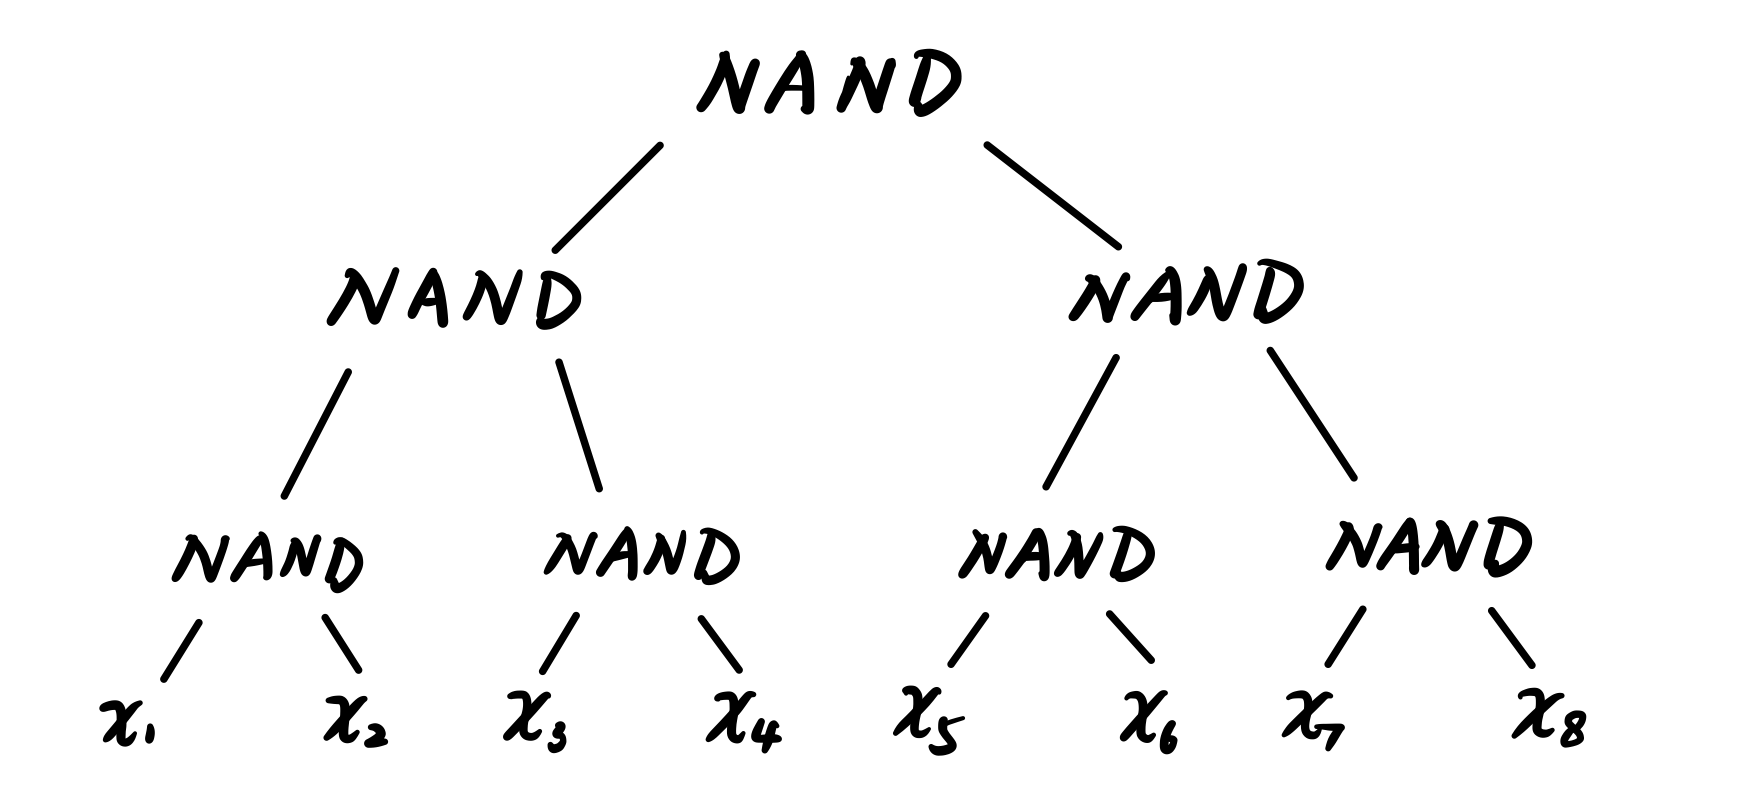
\includegraphics[scale = 0.15]{2/NAND tree.png}
\end{center}
We want to know the output of the root node. \\
Deterministically, the time complexity is $\Theta(n) = \Theta(2^h)$. \\
As for the randomized algorithm, we first consider a step of the algorithm, denoted as $\mathcal{A}_h$, where $h$ represents the height of the tree. This single step does one thing: starting from the root, examine left or right branch uniformly at random; if sees $0$, we output $1$; if sees $1$, we examine the other branch and the output NAND of both examinations. This is a recursive randomized algorithm. \\
We further denote $\alpha_b(h)$ to be the expected complexity of $\mathcal{A}_h$ if input $\mathbf{x}$ maps to $b$. \\
Then, we have:
\begin{align*}
    \alpha_0(h) &\le 2\alpha_1(h - 1) \\
    \alpha_1(h) &\le \max \begin{cases}
        \alpha_0(h - 1) \\
        \alpha_0(h - 1) + \frac{1}{2} \alpha_1(h - 1) \\
        \alpha_0(h - 1) + \frac{1}{2} \alpha_1(h - 1)
    \end{cases} \\
    &\le 2\alpha_1(h - 2) + \frac{1}{2}\alpha_1(h - 1)
\end{align*}
These inequalities stand from the NAND operations where:
\begin{align*}
    0 \text{ NAND } 0 &= 1 \\ 
    0 \text{ NAND } 1 &= 1 \\ 
    1 \text{ NAND } 0 &= 1 \\
    1 \text{ NAND } 1 &= 0
\end{align*}
And this algorithm solves to have a complexity of $\sim \order{1.686^h}$. \\
This is a type of \impt{Las Vegas} algorithm, where we have unfixed runtime, but the output is always correct.

\subsection{Randomized vs. Deterministic Algorithms}
A randomized algorithm can be thought of as choosing from some distribution of deterministic algorithms. If we require the randomized algorithms to have both fixed runtime and the output to be always correct, then there is no advantage from randomization. \\
We cover randomized algorithms because many quantum algorithms employ randomness and we want to show that quantum algorithms can be strictly faster than randomized algorithms (otherwise, speedup from randomization would be enough).

\subsection{Randomized State - 随机态}
\begin{definition}
    A \uimpt{randomized state} on $n$ bits is described by a column vector of length $2^n$
    $$\vec{p} = (p_{00 \dots 0}, p_{00 \dots 1}, \dots, p_{11 \dots 1})^\top$$
    such that it satisfies two conditions:
    \begin{quote}
        1. Normalization: $\Sumi{\mathbf{x}} p_{\mathbf{x}} = 1$. \\
        2. Non-negativity: $\forall p_{\mathbf{x}}, p_{\mathbf{x}} \ge 0$
    \end{quote}
\end{definition}
If exactly one of $p_{\mathbf{x}} \ne 0$, we refer to $\vec{p}$ as a \impt{deterministic state}, corresponding to bitstring $\mathbf{x}$. \\
Note that \impt{doing operations on randomized states in different orders can change the outcome}. We can also consider doing randomized operations on randomized states as well.

\subsection{Randomized Operation - 随机过程}
\begin{definition}
    A \uimpt{randomized operation} (a.k.a stochastic operation/matrix) acting on $n$ bits is described by a $2^n \times 2^n$ matrix $A$, such that:
    \begin{quote}
        1. All entries of $A$ are non-negative, \\
        2. Sum of every column is $1$.
    \end{quote}
\end{definition}
This implies that every column is a randomized state. If every column is a deterministic state, then we say $A$ is a \impt{deterministic operation}. \\
For example, a coin flip on $1$ bit can be characterized as
$$A = \begin{pmatrix}
    \frac{1}{2} & \frac{1}{2} \\
    \frac{1}{2} & \frac{1}{2}
\end{pmatrix}$$
\begin{lemma}
    A randomized operation that acts on a randomized state will yield a randomized state.
\end{lemma}

\subsection{Other Important Concepts}
The \impt{tensor product} of randomized states can be regarded as the following. Consider a $2$-bit state, where the first bit is determined by a fair coin, while the second bit is set to $0$. If we wish to describe the final state, we have:
$$\begin{pmatrix}
    \frac{1}{2} \\ \frac{1}{2}
\end{pmatrix} \otimes \begin{pmatrix}
    1 \\ 0
\end{pmatrix} = \begin{pmatrix}
    \frac{1}{2} \begin{pmatrix}
        1 \\ 0
    \end{pmatrix} \\ \frac{1}{2} \begin{pmatrix}
        1 \\ 0
    \end{pmatrix}
\end{pmatrix} = \begin{pmatrix}
    \frac{1}{2} \\ 0 \\ \frac{1}{2} \\ 0
\end{pmatrix}$$
Similarly, an example of the tensor product of randomized operations is the following:
$$\text{NOT} \otimes \id$$
A \impt{randomized circuit} is a circuit consisting of randomized operations. \\
\impt{Measuring a randomized state} on $n$ bits, $\vec{p}$, is a procedure that outputs $\mathbf{x} \in \{0, 1\}^n$ with probability $p_{\mathbf{x}}$. \\
The process of randomized computation consists of input bits and \impt{ancillas} that goes through a randomized circuit and obtain an output through a measurement. \\
For randomized computation, the Toffoli gate and the CNOT operation is universal -- any randomized computation can be decomposed into a sequence of these 2 operations to arbitrary precision.

\newpage
\section{Basics of Quantum Information Processing - 量子信息处理初步}
\subsection{Complex Numbers - 复数}
Let $a, b, c, d, r, \theta \in \R$, we introduce the imaginary unit $\imag$ where $\imag^2 = -1$. \\
A complex number is in the form of $z = a + b\imag$ with the following arithmetic properties:
\begin{align*}
    (a + b\imag)(c + d\imag) &= (ac - bd) + (ad + bc)\imag \\
    \abs{a + b\imag} &= \sqrt{a^2 + b^2} \\
    e^{\imag \theta} &= \cos \theta + \imag \sin \theta \\
    \conj{(a + b \imag)} &= a - b\imag
\end{align*}
Let $z, z_1, z_2 \in \C$, then we have:
\begin{align*}
    \abs{z}^2 &= z \cdot \conj{z} \\
    z_1 &= r_1 e^{\imag \theta_1} \\
    z_2 &= r_2 e^{\imag \theta_2} \\
    z_1z_2 &= (r_1r_2) e^{\imag (\theta_1  + \theta_2)}
\end{align*}

\subsection{Quantum State - 量子态}
\begin{definition}
    A quantum state of $n$ qubits is described by a column vector of length $2^n$,
    $$\vec{\alpha} = (\alpha_{00 \dots 0}, \alpha_{00 \dots 1}, \dots, \alpha_{11 \dots 1})^\top$$
    such that $\alpha_{\mathbf{x}} \in \C$, and $\Sumi{\mathbf{x}} \abs{\alpha_{\mathbf{x}}}^2 = 1$.
\end{definition}
It is easy to see any deterministic state is a quantum state.

\subsection{Kronecker Product and Dirac Notation}
\begin{definition}
    Let $A \in \C^{m_1 \times m_2}$ and $B \in \C^{n_1 \times n_2}$, then
    $$A \otimes B = \begin{pmatrix}
        a_{11}B & a_{12}B & \cdots & a_{1,m_2}B \\
        a_{21}B & a_{22}B & \cdots & a_{2,m_2}B \\
        \vdots & \vdots & \ddots & \vdots \\
        a_{m_11}B & a_{m_1, 2}B & \cdots & a_{m_1,m_2}B
    \end{pmatrix} \in \C^{(m_1 \times n_1)(m_2 \times n_2)}$$
\end{definition}
It is conventional to write $\vec{\alpha}$ as $\ket{\alpha}$:
$$\ket{\alpha} = \Sumi{\mathbf{x}} \alpha_{\mathbf{x}} \ket{x_1 x_2 \cdots x_n}$$
In $\C^d$ for $d > 2$, it is conventional to write:
$$\ket{0} = \begin{pmatrix}
    1 \\ 0 \\ \vdots \\ 0
\end{pmatrix}, \ket{1} = \begin{pmatrix}
    0 \\ 1 \\ \vdots \\ 0
\end{pmatrix}, \ket{d - 1} = \begin{pmatrix}
    0 \\ 0 \\ \vdots \\ 1
\end{pmatrix}$$
The properties of the Kronecker product consists of the following:
\begin{quote}
    Let $A, B, C, D \in \C^{m \times n}$, and let $\alpha, \beta \in \C$. \\
    1. Bilinearity: if $A$ and $B$ have same dimensions, $$C \otimes (\alpha A + \beta B) = \alpha C \otimes A + \beta C \otimes B$$
    2. Associativity $$(A \otimes B) \otimes C = A \otimes (B \otimes C)$$
    3. Mixed product: if $A, C$ have same dimensions, and $B, D$ have same dimensions
    $$(A \otimes B)(C \otimes D) = AC \otimes BD$$
\end{quote}
With these setup, we can see that if $A \in \C^{d \times d}$, then
$$A \ket{i} = \Sum{j = 1}{d} A_{ji} \ket{j}$$
for all $i \in \{1, \dots, d\}$.

\subsection{Quantum Operations - 量子操作}
\begin{definition}
    A square matrix $\opuni$ is \uimpt{unitary} if $\conjt{\opuni}\opuni = \id$.
\end{definition}
\begin{lemma}
    $\ket{u_1}, \ket{u_2}, \dots, \ket{u_d} \in \C^d$ form an orthonormal basis if there exists a unitary matrix $\opuni$ such that $\ket{u_i} = \opuni \ket{i}$
\end{lemma}
\begin{definition}
    A \uimpt{quantum operation} on $d$-dimensional quantum states is described by a $d \times d$ unitary matrix.
\end{definition}
Common elementary gates include
$$H = \frac{1}{\sqrt{2}}\begin{pmatrix}
    1 & 1 \\
    1 & -1
\end{pmatrix}, X = \begin{pmatrix}
    0 & 1 \\
    1 & 0
\end{pmatrix}, Y = \begin{pmatrix}
    0 & -\imag \\
    \imag & 0
\end{pmatrix}, Z = \begin{pmatrix}
    1 & 0 \\
    0 & -1
\end{pmatrix}, T = \begin{pmatrix}
    1 & 0 \\
    0 & e^{\imag \frac{\pi}{4}}
\end{pmatrix}, \text{CNOT}, \text{Toffoli}$$
where $H$ is the \impt{Hadamard} gate, and $X, Y, Z$ are \impt{Pauli gates}.

\subsection{Quantum Circuit - 量子电路}
\begin{definition}
    A \uimpt{quantum circuit} is a sequency of quantum operations.
\end{definition}
\begin{definition}
    \uimpt{Measuring a quantum state} of $n$-qubits \impt{in the quantum basis} $\ketpsi = \Sumi{\mathbf{x}} \alpha_{\mathbf{x}}\ket{\mathbf{x}}$ refers to a process that returns an $n$-bit classical string $\mathbf{x} \in \{0, 1\}^n$ with probability $\abs{\alpha_{\mathbf{x}}}^2$.
\end{definition}
Common universal gate sets for a quantum circuit include
$$\{H, \text{CNOT}, T\}, \{H, \text{Toffoli}\}$$

\subsection{Unitary Matrix in Quantum Computation - 量子计算中的酉矩阵}
We refer the \impt{bra} notation to be row vectors (e.g. $\brapsi$) and \impt{ket} notation to be column vectors (e.g. $\ketpsi$). Let $\ketpsi,\ketphi \in \C^d$, we have $\brapsi = \conjt{\ketpsi}, \braket{\phi}{\psi} = \brapsi \cdot \ketpsi$. The norm of $\ketpsi$ is $\norm{\ketpsi} = \sqrt{\braket{\psi}}$.
\begin{lemma}
    For operations $\text{op} \in \{*, \top, \dagger\}$, we have
    \begin{align*}
        (A + B)^{\text{op}} &= A^{\text{op}} + B^{\text{op}} \\
        (A \otimes B)^{\text{op}} &= A^{\text{op}} \otimes B^{\text{op}}
    \end{align*}
    and $\conj{(AB)} = \conj{A}\conj{B}$, $(AB)^\top = B^\top A^\top$, $\conjt{(AB)} = \conjt{B}\conjt{A}$
\end{lemma}
\begin{lemma}
    Suppose $\ketpsi = \Sum{i = 1}{d} \alpha_i \ket{i} \in \C^d$, then $\ketpsi$ is a quantum state if and only if $\braket{\psi} = 1$.
\end{lemma}
\begin{theorem}
    Let $\ket{u_1}, \ket{u_2}, \dots, \ket{u_d} \in \C^d$, then $\braket{u_i}{u_j} = \delta_{ij}$ for all $i, j \in \{1, \dots, d\}$ if and only if they form an orthonormal basis. \\
    Equivalently, a $d \times d$ matrix is unitary if and only if the columns of $A$ are unit vectors and are pair-wise orthogonal.
\end{theorem}
\begin{theorem}
    A $d \times d$ complex matrix $A$ maps a $d$-dimensional quantum state to another $d$-dimensional quantum state if and only if $A$ is unitary.
\end{theorem}

\newpage
\section{CHSH Game}
The CHSH game, also demonstrating the violation of Bell inequality, has the following set up. \\
We have $3$ people, Alice, Bob and the referee. The referee will distribute $x, y$ to Alice and Bob respectively such that $x, y$ are drawn uniformly at random from the set $\{0, 1\}$. Without discussing, Alice and Bob must give $a, b \in \{0, 1\}$ to the referee respectively in their own choices. Alice and Bob wins if
$$a \oplus b = x \land y$$
One na\"ive strategy that Alice and Bob can use is always choosing $a = b = 0$, this way they have a $\frac{3}{4}$ chance of winning the game. \\
If we think about it more generally, and discuss a deterministic strategy, that is:
\begin{align*}
    a: \{0, 1\} &\to \{0, 1\} \\
    x &\mapsto 0 \text{ or } 1 \\
    b: \binset &\to \binset \\
    y &\mapsto 0 \text{ or } 1
\end{align*}
We can demonstrate that for all possible pairs of $(x, y)$, it is impossible to satisfy $a(x) \oplus b(y) = x \land y$ at the same time. There is at most a $\frac{3}{4}$ chance of winning the game. \\
What if we employ a randomized strategy? Before Alice and Bob go into the game, they sample some random variable $\lambda \in \R$ with probability density $p_\lambda$, and choose a deterministic strategy $a_\lambda$ and $b_\lambda$. If we draw out each $\lambda_i$ for all $i \in \{1, \dots, n\}$, each path is a deterministic strategy with winning probability at most $\frac{3}{4}$. Thus, the probability of winning the game using randomized strategy:
$$\Prob{\text{winning}} \le \Sumi{i} p_{\lambda_i} \times 0.75 = 0.75$$
Thus, any \impt{randomized strategy} with \impt{no communication} wins with a probability at most $0.75$; any \impt{hidden variable} theory that is also \impt{local} wins with a probability at most $0.75$.

\subsection{Quantum Strategy - 量子策略}
\begin{theorem}
    By employing a quantum strategy, Alice and Bob can win the game with probability $\cos^2(\frac{\pi}{8})$.
\end{theorem}
\begin{definition}
    A $2$-qubit state $\ketpsi$ is \uimpt{entangled} if $\ketpsi$ cannot be written as $\ket{\psi_1} \otimes \ket{\psi_2}$ where $\ket{\psi_i}$ are $1$-qubit states.
\end{definition}
The quantum strategy is described by a quantum circuit:
\begin{center}
    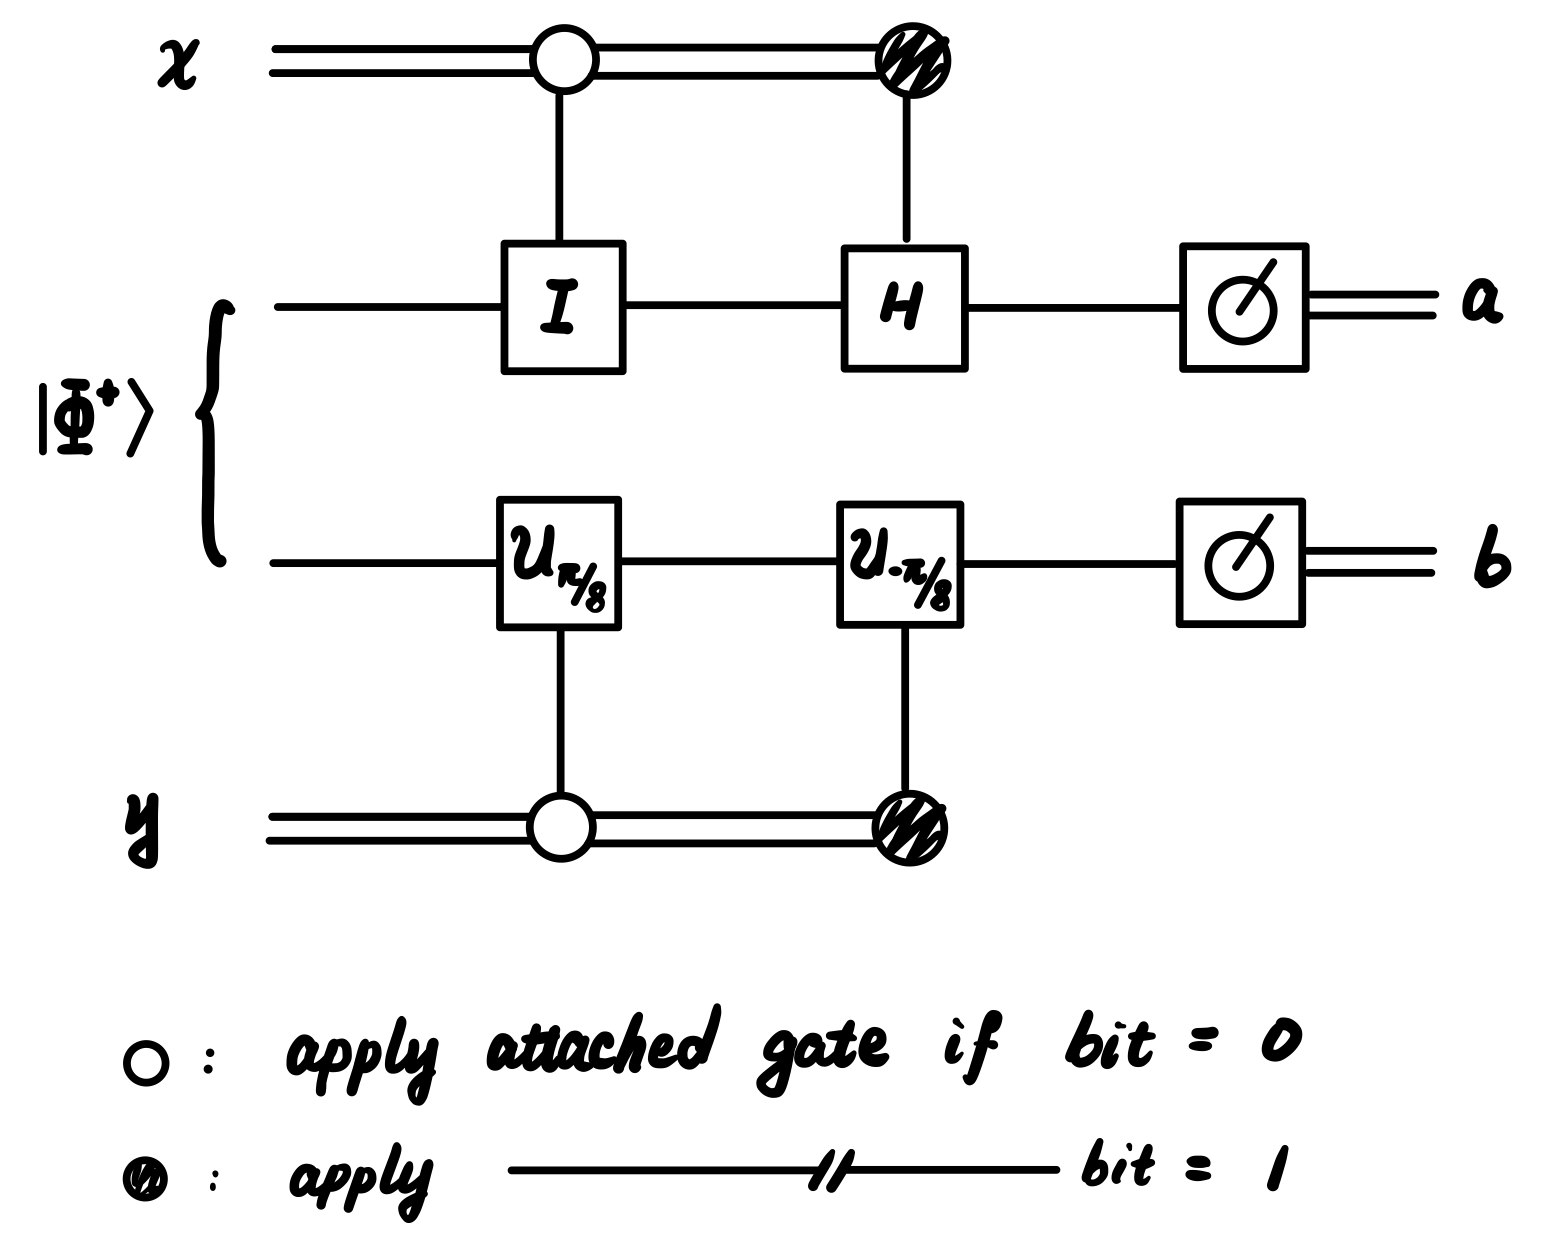
\includegraphics[scale=0.2]{4/chsh.png}
\end{center}
where $\opuni_\theta$ is the following (it can be interpreted as a rotation matrix by angle $\theta$ \impt{clockwise}):
$$\opuni_\theta = \begin{pmatrix}
    \cos \theta & \sin \theta \\
    -\sin \theta & \cos \theta
\end{pmatrix}$$
and $\ket{\Phi^+}$ is also called the EPR pair specified to be:
$$\ket{\Phi^+} = \frac{1}{\sqrt{2}}(\ket{00} + \ket{11})$$
We provide one example case to demonstrate the above probability, where $x = 1$ and $y = 0$:
\begin{align*}
    \ket{\Phi^+} &\to (H \otimes \opuni_{\frac{\pi}{8}}) \\
    &= \id(H \otimes \opuni_{\frac{\pi}{8}})\ket{\Phi^+} \\
    &= \Sumi{\mathbf{x}} \dyad{\mathbf{x}} H \otimes \opuni_{\frac{\pi}{8}} \ket{\Phi^+} \\
    &= \Sumi{\mathbf{x}} \mel{\mathbf{x}}{H \otimes \opuni_{\frac{\pi}{8}}}{\Phi^+}\ket{\mathbf{x}}
\end{align*}
Since $x \land y = 0$, we want $a \oplus b = 0$, meaning that either $a = b = 0$ or $a = b = 1$, that is, we only care about the coefficients for $\mathbf{x} = 00, 11$, which is:
$$\Prob{\mathbf{x} = 00, \mathbf{x} = 11} = \abs{\mel{00}{H \otimes \opuni_{\frac{\pi}{8}}}{\Phi^+}}^2 + \abs{\mel{11}{H \otimes \opuni_{\frac{\pi}{8}}}{\Phi^+}}^2$$
If we expand the first part we have:
\begin{align*}
    \mel{00}{H \otimes \opuni_{\frac{\pi}{8}}}{\Phi^+} &= \frac{1}{\sqrt{2}} \bra{00} (H \otimes \opuni_{\frac{\pi}{8}} \ket{00} + H \otimes \opuni_{\frac{\pi}{8}} \ket{11}) \\
    &= \frac{1}{\sqrt{2}} \bra{00} ((\frac{1}{\sqrt{2}}(\ket{0} + \ket{1}))(\cos\theta\ket{0} - \sin\theta\ket{1}) \\
    &+ (\frac{1}{\sqrt{2}}(\ket{0} - \ket{1}))(\sin\theta\ket{0} + \cos\theta\ket{1})) \\
    &= \frac{1}{2} (\cos\theta + \sin\theta)
\end{align*}
If we do the same thing for $\mel{11}{H \otimes \opuni_{\frac{\pi}{8}}}{\Phi^+}$, we would obtain $\frac{1}{2}(-\sin\theta - \cos\theta)$.
We take the square of each value, add them together, and substitute $\theta = \frac{\pi}{8}$, we get the probability of $\cos^2(\frac{\pi}{8})$.

\subsection{Partial Measurement - 部分测量}
\begin{definition}
    Let $m \le n$ be positive integers. A \uimpt{partial measurement} of the first $m$ qubits of an $n$-qubit state $\ketpsi = \Sumi{\mathbf{x}}\alpha_{\mathbf{x}} \ket{\mathbf{x}}$ is a process that: \\
    1. returns $\mathbf{y} \in \binset^m$ with probability
    $$p_{\mathbf{y}} := \norm{(\bra{\mathbf{y}} \otimes \id^{n - m})\ketpsi}^2 = \Sumi{\mathbf{x}[1:m] = \mathbf{y}} \abs{\alpha_{\mathbf{x}}}^2$$
    2. given $\mathbf{y}$ is returned, the state of the remaining $n - m$ qubits become
    $$\ket{\psi_\mathbf{y}} := \frac{\mel{\mathbf{y}}{\id^{n-m}}{\ketpsi}}{\sqrt{p_{\mathbf{y}}}}$$
\end{definition}
An example of this is given $\ketpsi = \sqrt{\frac{1}{2}} \ket{00} + \sqrt{\frac{1}{4}} \ket{01} + \sqrt{\frac{1}{6}} \ket{10} + \sqrt{\frac{1}{12}} \ket{11}$, if we measure the $1^{st}$ qubit, the probability of getting $0$ is $\frac{3}{4}$ and getting $1$ to be $\frac{1}{4}$, which both coincidentally have the same leftover state after partial measurement to be:
$$\sqrt{\frac{2}{3}}\ket{0} + \sqrt{\frac{1}{3}}\ket{1}$$
\begin{theorem}
    Let $\ketphi$ bet any $n$-qubit state, consider $2$ experiments:
    1. directly measure the first $m$ qubits, obtaining outcome $b$ and post-measurement state $\ket{\phi_b}$. \\
    2. first apply some $(n-m)$-qubit unitary $\opuni$ on the last $n-m$ qubits of $\ketphi$, then measure the first $m$ qubits of $\ketphi$, obtaining outcome $c$ and post-measurement state $\ket{\phi_c'}$. \\
    Then, the distribution of $b, c$ are identical, and $\ket{\phi_c'} = \opuni \ket{\phi_c}$ for all $c \in \binset^m$.
\end{theorem}

\subsection{Alternative Analysis}
Given the partial measurement definition, we can re-analyze the CHSH game. \\
From linear algebra, for two real vectors $\ket{u}$ and $\ket{v}$ of the same dimension, we have:
$$\braket{u}{v} = \norm{\ket{u}} \cdot \norm{\ket{v}} \cdot \cos \theta$$
and if they are quantum states, we further have $\abs{\braket{u}{v}}^2 = \cos^2\theta$. \\
We can consider that Alice measuring first, which is a partial measurement on the first qubit, and get $a$.
For each case of $(x, y)$, we can then consider the probability of Bob measuring the corresponding $b$ so that they can win to be plotted on a 2D Cartesian plane. \\
An example of this is when $(x, y) = (0, 0)$, Alice has $\frac{1}{2}$ of getting $0$ and $1$ respectively. And we want to find the probability of Bob measuring $0$ and $1$ respectively as well, then we have:
\begin{center}
    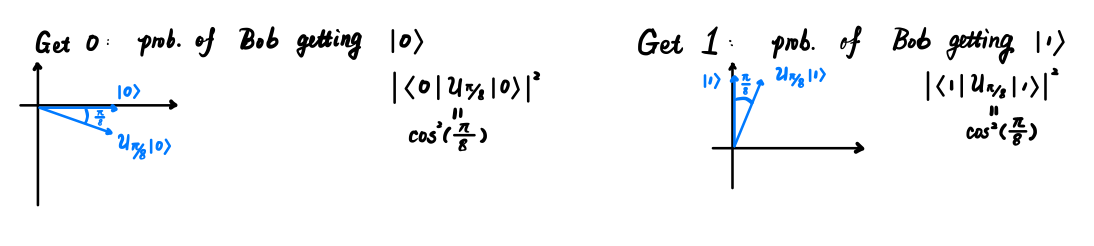
\includegraphics[scale = 0.4]{4/chsh_alt.png}
\end{center}
This process can be applied to each $(x, y)$.

\newpage
\section{Deutsch's Problem}
We wish to explore quantum algorithms and speedups. The first historic example of quantum speedup is from Deutsch's problem. The setup of this problem is as follows. \\
Given $f: \binset \to \binset$, we ask if $f$ is balanced ($f(0) \ne f(1)$) or constant ($f(0) = f(1)$). \\
From here, we give some what we mean by comparing the complexity between classical algorithms and quantum algorithms. \\
For a classical algorithm, we assume $f$ can only be accessed through queries (which is an evaluation of $f$ at a single point), and each query is unit cost. The complexity of the algorithm is the number of queries needed to solve the problem. To solve the above problem with certainty, $2$ queries is needed. \\
For a quantum algorithm, assume we have the ability to apply a $2$-qubit unitary at unit cost, defined by
$$O_f: \ket{\mathbf{x}} \ket{b} \mapsto \ket{\mathbf{x}} \ket{b \oplus f(x)}$$
for all $\mathbf{x}, b \in \binset$. Each application of $O_f$ is a quantum query to $f$. To solve the above problem with certainty, only $1$ quantum query is needed. \\
The quantum circuit is set up as the following:
\begin{center}
    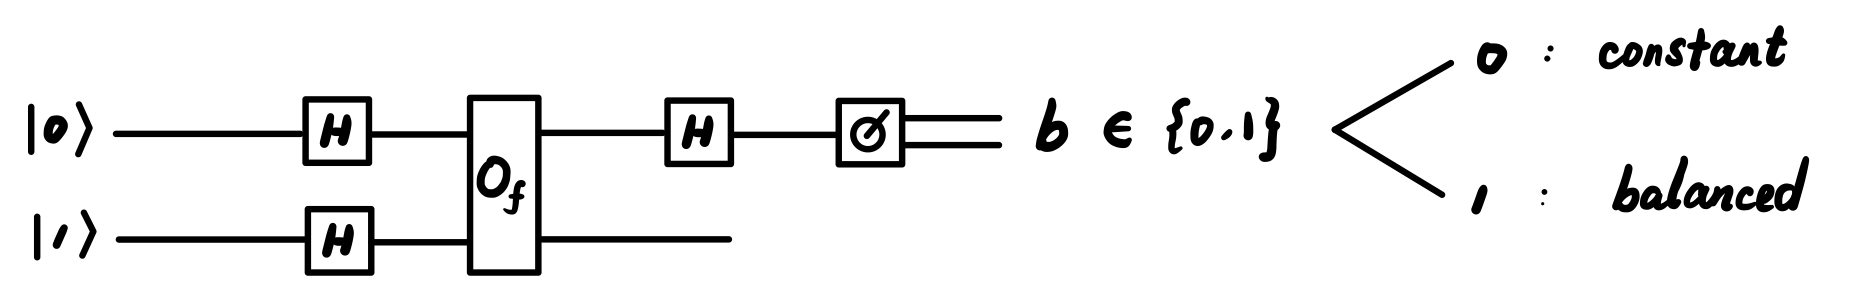
\includegraphics[scale = 0.2]{5/deutsch.png}
\end{center}
During this analysis, two mathetical relations is useful:
$$\ket{0 \oplus x} = \ket{x}$$
$$\ketx - \ket{1 \oplus x} = (-1)^x(\ket{0} - \ket{1})$$
The above circuit, with a single quantum query, can solve Deutsch's problem, the mathematical derivation is not included.
We may also think of this from a partial measurement perspective, where applying a unitary on the non-measured qubit does not change the probability distribution of the measured qubit, so if we apply another Hadamard gate after the quantum query on the second qubit, we can simplify the state before measurement to be:
$$\ket{\psi'} = (-1)^{f(0)} \begin{cases}
    \ket{0} & \text{constant} \\
    \ket{1} & \text{balanced}
\end{cases} \otimes \ket{1}$$

\subsection{Quantum Oracle}
Given $f$ as a classical circuit, we can systematically and efficiently convert a classical circuit diagram into its corresponding quantum oracle.
\begin{definition}
    Let $f: \binset^m \to \binset^n$, the \uimpt{quantum oracle} of $f$ is the unitary matrix $O_f \in \C^{2^{m+n} \times 2^{m + n}}$ defined by
    $$O_f: \ket{\mathbf{x}}\ket{\mathbf{y}} \mapsto \ket{\mathbf{x}}\ket{\mathbf{y} \oplus f(\mathbf{x})}$$
\end{definition}
\begin{theorem}
    Any $f$ can be implemented as a classical circuit involving FANOUT, NOT, AND, OR gates.
\end{theorem}
\begin{theorem}
    Suppose we have the description of classical circuit implementing $f$ in terms of the above gates, we can systematically and efficiently implement $O_f$ using CNOT, X, and Toffoli gates. \\
    More precisely, the implementation takes size that is linear (roughly $2\times$ due to symmetry) in the size (number of gates) of the classical circuit.
\end{theorem}
Specifically, we map FANOUT to CNOT gate, NOT to X gate, AND to Toffoli gate, and OR can be implemented using Toffoli and X gates (because OR can be implemented using NAND gates). An example is the following:
\begin{center}
    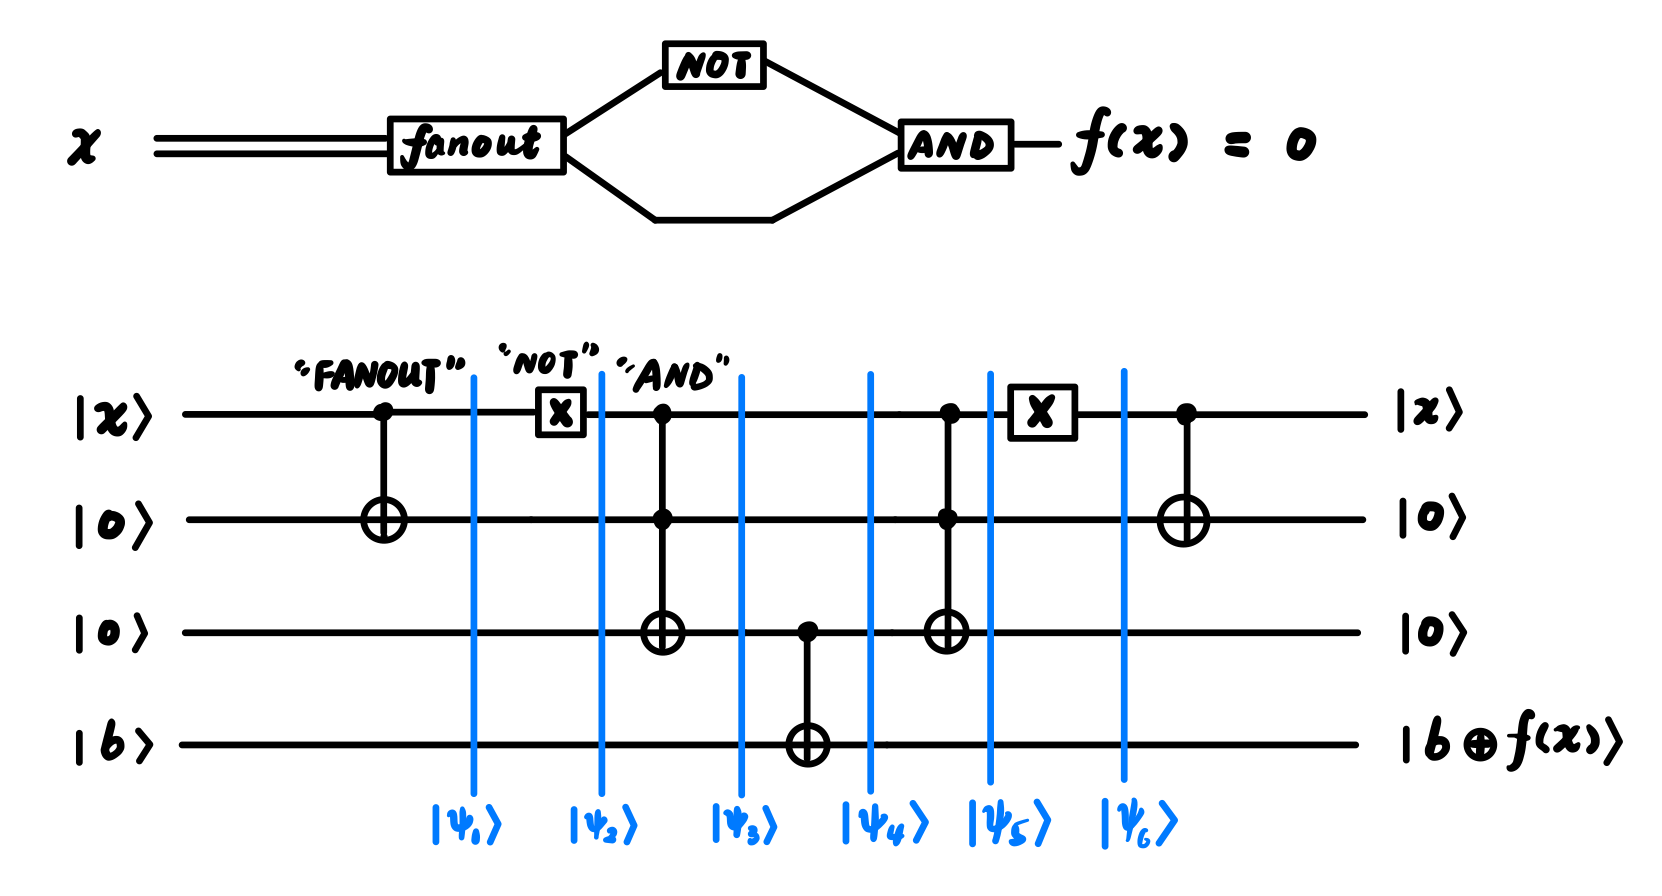
\includegraphics[scale = 0.2]{5/oracle.png}
\end{center}
We can consider CNOT ``copying'' a bit (because $0 \oplus x = x$), X negates a bit (because X maps $\ket{0}$ to $\ket{1}$ and vice versa), Toffoli taking two bits and put the AND result into the third bit (because Toffoli only flips the third bit if both first bit and second bit are $1$).

\newpage
\section{Deutsch-Jozsa Problem}
Deutsch-Jozsa is an ``upgraded'' version of Deutsch's problem. The problem set up is the following. \\
Given $f: \binset^n \to \binset$, we are \impt{promised} that it is either constant ($\forall \mathbf{x} \in \binset^n, f(\mathbf{x}) = b$) or balanced (half of $\mathbf{x} \in \binset^n, f(\mathbf{x}) = 0$, the other half gives $1$). We want to decide which case we are in. \\
The quantum circuit that solves this problem is the following:
\begin{center}
    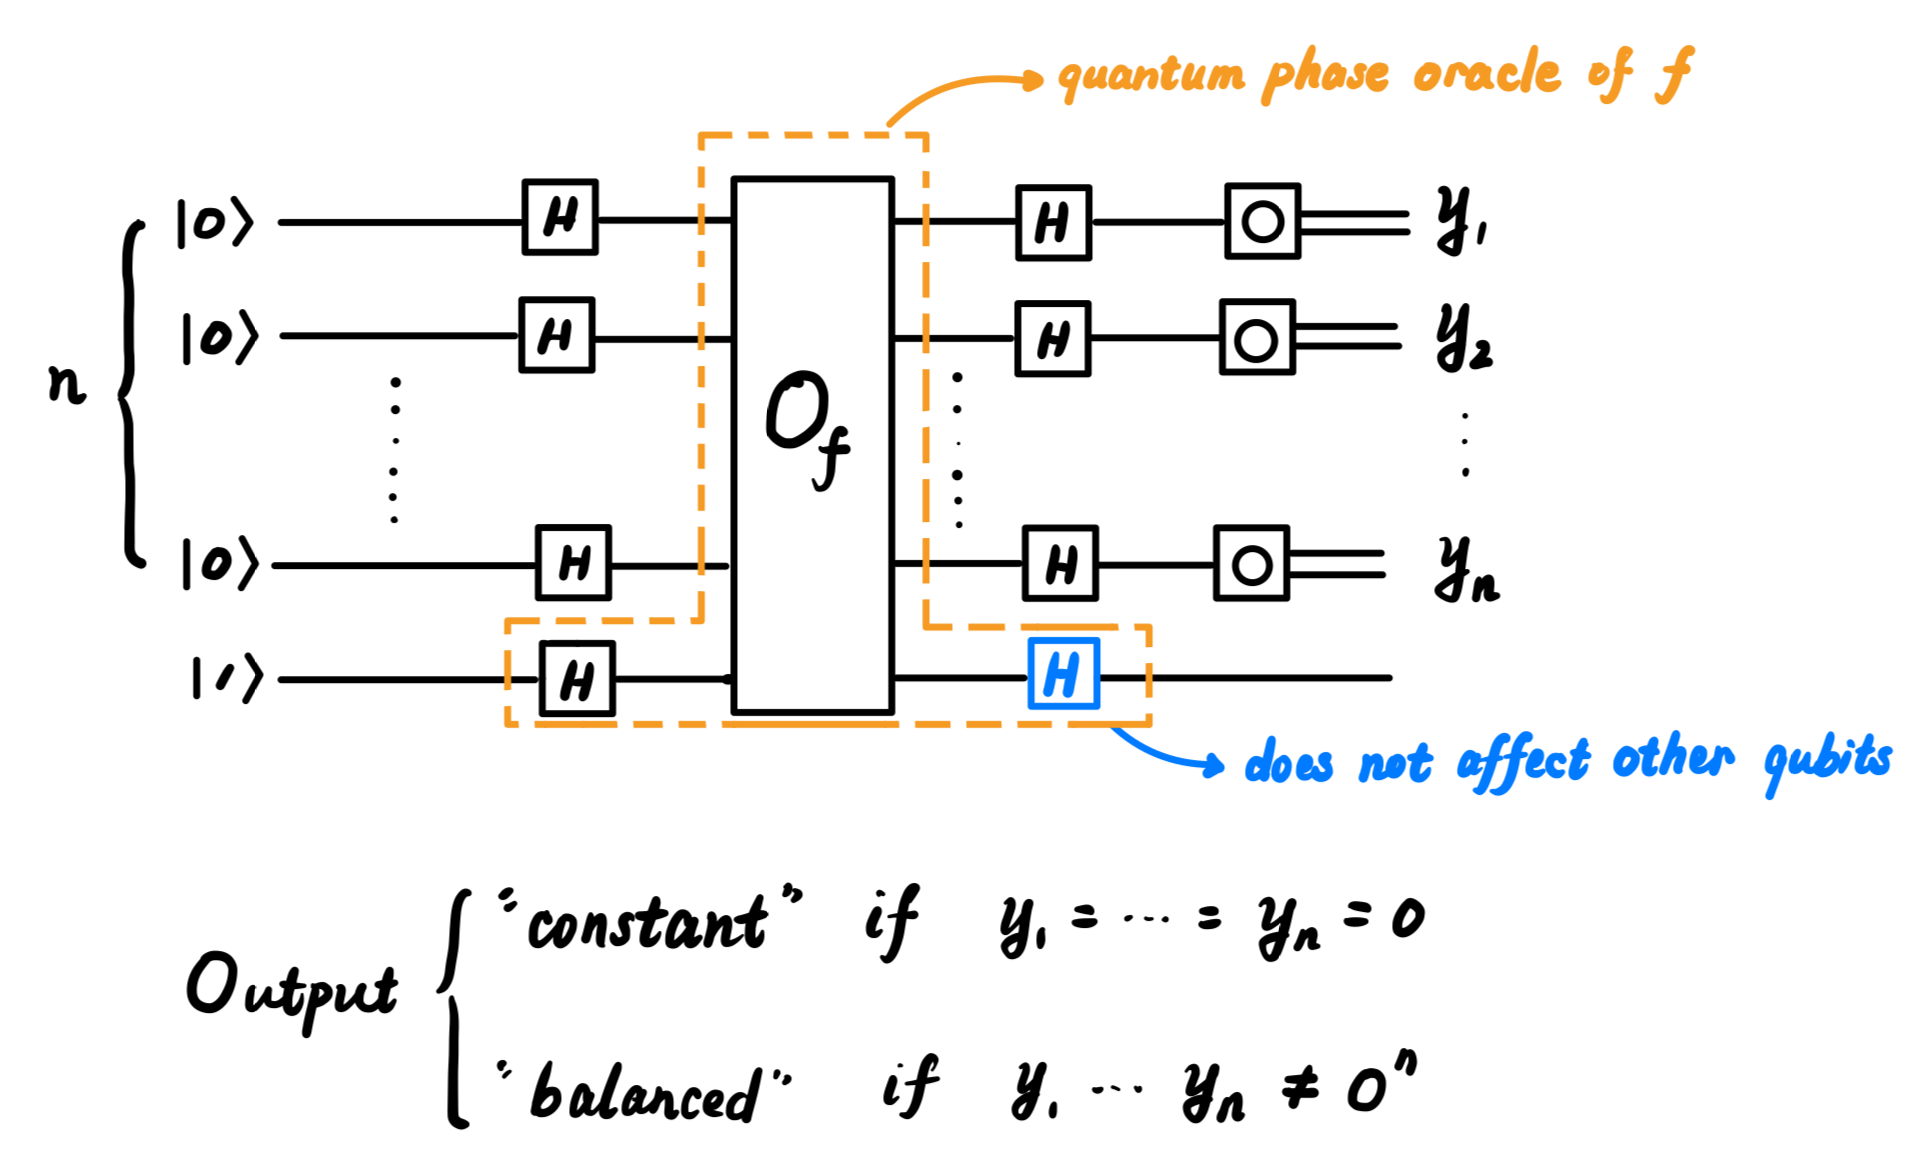
\includegraphics[scale = 0.2]{6/deutsch-jozsa.png}
\end{center}
The \impt{quantum phase oracle} of $f$ mentioned in this circuit is given by:
$$\opuni_f: \mathbf{x}\ket{b} \mapsto (-1)^{b \cdot f(\mathbf{x})}\ket{\mathbf{x}}\ket{b}$$
One useful lemma for analysis is that
\begin{lemma}
    Given $b \in \binset$, we have
    $$H\ket{b} = \frac{1}{\sqrt{2}}(\ket{0} + (-1)^b\ket{1}$$
    This extends to
    $$H^n \ket{\mathbf{x}} = \frac{1}{\sqrt{2^n}} \Sumi{\mathbf{y} \in \binset^n} (-1)^{\mathbf{x} \cdot \mathbf{y}}\ket{\mathbf{y}}$$
    where
    $$\mathbf{x} \cdot \mathbf{y} = \Sum{i = 1}{n} x_i \cdot y_i$$
\end{lemma}
Another useful mathematical trick is that
$$(-1)^{1 \oplus b} = -(-1)^b$$
where $b \in \binset$. \\
The speedup of this quantum circuit is obvious. If we use a classical query model, we need $2^{n-1} + 1$ times to be certain. In this model, we need one quantum query to be certain. \\
However, this \impt{does not} mean we have an unconditional provable exponential quantum speedup, becuase once we instantiate $f$ as a classical circuit, there may be more efficient ways of solving the D-J problem classically, by analyzing the circuit and just querying it. \\
Being only able to query the circuit for $f$ is the essential simplifying assumption of the query model.


\newpage
\section{Simon's Problem}
Simon's problem gives an exponential separation between classical and quantum without demanding certain correctness. \\
In some sense, the problem remains hard classically and easy quantumly, even when the oracle is instantiated as a circuit as far as we know: because Shor's algorithm is ``in some sense'' Simon's problem but with the oracle instantiated as a specific circuit. \\
The setup for the problem is the following. For $n \in \N$, let:
\begin{align*}
    \mathcal{D}_0 &:= \{f: \binset \to \binset \mid f \text{ is a bijection}\} \\
    \mathcal{D}_1 &:= \{f: \binset \to \binset \mid \exists! \mathbf{s} \in \binset^n - \{0\}^n, \forall \mathbf{x} \in \binset^n, f(\mathbf{x}) = f(\mathbf{x} \oplus \mathbf{s})\}
\end{align*}
That is, in the case of $\mathcal{D}_1$, if $f(\mathbf{x}) = f(\mathbf{y})$, then $\mathbf{y} \in \{\mathbf{x}, \mathbf{x} \oplus \mathbf{s}\}$, where $\mathbf{s}$ is a unique non-zero bitstring. An example of this is:
\begin{center}
    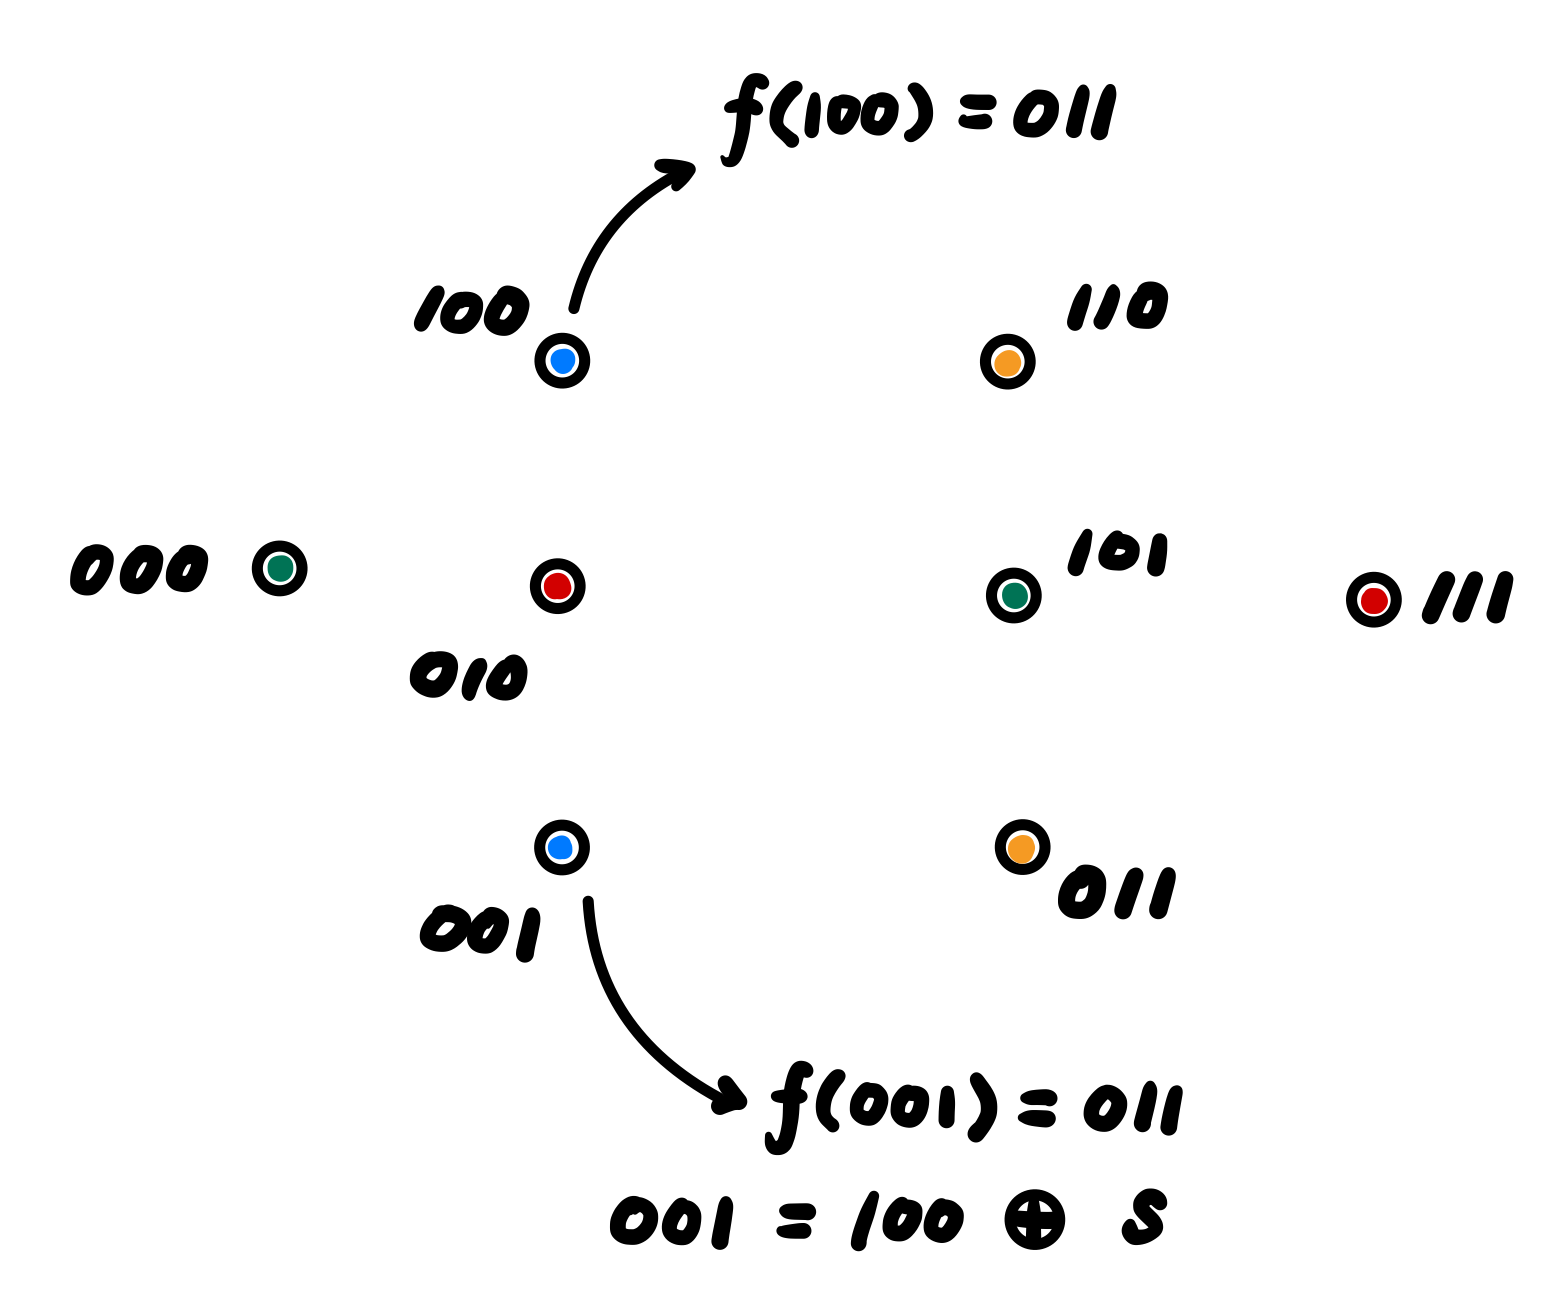
\includegraphics[scale = 0.2]{7/d1_example.png}
\end{center}
where $\mathbf{s} = 101$. We can view this function as a coloring with $2^{n-1}$ colors with each color covering exactly two inputs. Each color represent an output. \\
We want to decide which case $f$ is in, given query access to $f$, \impt{promised} one of the cases hold (but we do not know $\mathbf{s}$). \\
Classically, we need $2^{n-1} + 1$ queries to deterministically solve the problem. When employing a randomized algorithm, the time complexity is $\Theta(\sqrt{2^n})$, which is related to the ``birthday paradox''.

\subsection{Quantum Strategy}
In the quantum case, we only need $\order{n}$ queries and give the correct answer with high probability. The circuit is as follows:
\begin{center}
    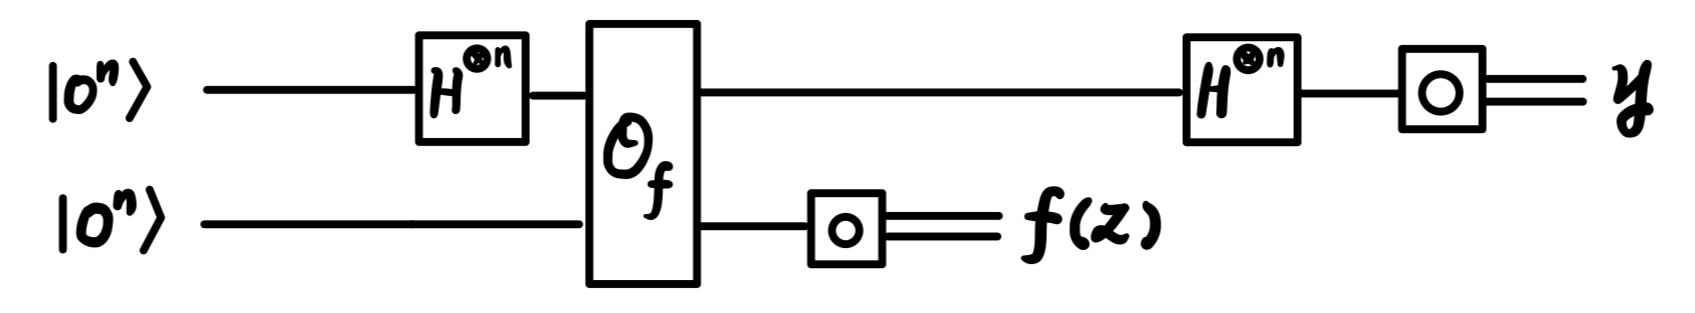
\includegraphics[scale = 0.2]{7/circuit.png}
\end{center}
We measure the last $n$ qubits, and obtain $f(\mathbf{z})$. If $f \in \mathcal{D}_0$, the state of first $n$ qubits collapes to $\ket{\mathbf{z}}$. If $f \in \mathcal{D}_1$, the state of first $n$ qubits collapses to $\frac{1}{\sqrt{2}}(\ket{\mathbf{z}} + \ket{\mathbf{z} \oplus \mathbf{s}})$. \\
Then, after applying $H^n$, if $f \in \mathcal{D}_0$, then we have:
$$\ket{\mathbf{z}} \mapsto \frac{1}{\sqrt{2^n}} \Sumi{\mathbf{y}} (-1)^{\mathbf{y} \cdot \mathbf{z}} \ket{\mathbf{y}}$$
if $f \in \mathcal{D}_1$, then:
$$\frac{1}{\sqrt{2}}(\ket{\mathbf{z}} + \ket{\mathbf{z} \oplus \mathbf{s}}) \mapsto \frac{1}{\sqrt{2^{n+1}}} (\Sumi{\mathbf{y}} (-1)^{\mathbf{y} \cdot \mathbf{z}}(1 + (-1)^{\mathbf{y} \oplus \mathbf{s}})\ket{\mathbf{y}})$$
This means, if we measure the first $n$ qubits, if $f$ is in the first case, each $\mathbf{y}$ has uniform probability of being measured. If $f$ is in the second case, then:
\begin{quote}
    1. $\mathbf{y} \cdot \mathbf{s} \equiv 0 \pmod 2$: $\Prob{\mathbf{y}} = \frac{1}{2^{n - 1}}$. \\
    2. $\mathbf{y} \cdot \mathbf{s} \equiv 1 \pmod 2$: $\Prob{\mathbf{y}} = 0$
\end{quote}
which is uniform over $\{\mathbf{y} \in \binset^n \mid \mathbf{y} \cdot \mathbf{s} \equiv 0 \pmod 2\}$. \\
Repeat the above process $K = \Theta(n) > n$ times to generate $K$ $\mathbf{y}$'s. Collect these $\mathbf{y}$'s into a $K \times n$ matrix:
$$A = \begin{pmatrix}
    \mathbf{y}_1 \\ \mathbf{y}_2 \\ \vdots \\ \mathbf{y}_K
\end{pmatrix}$$
and compute the rank of $A$ over $\F_2$. If the rank is $n$, output $\mathcal{D}_0$, if the rank is $< n$, output $\mathcal{D}_1$.

\begin{definition}
    For a matrix $A$ in $\F_2$, its rank is the \uimpt{minimal non-negative} $d$ such that the set of rows of $A$ can be expressed as 
    $$\{\beta_1 \vecv_1 \oplus \beta_2 \vecv_2 \oplus \cdots \beta_d \vecv_d \mid \beta_1, \beta_2, \dots, \beta_d \in \binset\}$$
    for some zero-one $\vecv_1, \dots, \vecv_d$.
\end{definition}
For example, take $\vecv_1 = (1, 0, 1)$ and $\vecv_2 = (1, 1, 0)$, by iterating through $\beta_1, \beta_2 \in \binset$, we can obtain $3$ non-zero vectors. \\
This gives that the algorithm is always correct in $\mathcal{D}_1$. \\
However, for $f \in \mathcal{D}_0$, we have:
\begin{lemma}
    $$\Prob{\rank A = n} \ge 1 - 2^{n - K}$$
\end{lemma}
Additionally, $\mathbf{s}$ can be computed from $\ker A$.

\newpage
\section{Shor's Algorithm}
\subsection{Modulo Operations and Relevant Mathematical Background}
\begin{definition}
    A prime number $p \in \Z^+$ is a number that has no divisors other than $1$ and $p$.
\end{definition}
\begin{theorem}
    The \uimpt{Fundamental Theorem of Arithmetic} states that for all positive integers $x$, $x$ can be factored into a product of primes. Moreover, the factorization is unique (up to re-ordering).
\end{theorem}
Given a positive interger $N$, let $x, y \in \Z$, we write
$$x \bmod N$$
to mean the unique element $x' \in \{0, \dots, N-1\}$ such that $N$ divides $(x - x')$. \\
We write
$$x \equiv y \pmod N$$
to mean that $x \bmod N = y \bmod N$.
\begin{definition}
    Given $a, b \in \Z$, not both zero, the \uimpt{greatest common divisor} of $a$ and $b$ is the largest $d \in \Z^+$ such that $d$ divides $a$ and $d$ divides $b$. We write:
    $$\gcd(a, b) = d$$
\end{definition}
\begin{definition}
    $a, b$ are co-prime if $\gcd(a, b) = 1$.
\end{definition}
\begin{definition}
    Let $a, N \in \Z^+$, if $\gcd(a, N) = 1$, and $\exists r \in \Z^+$ where $a^r \equiv 1 \pmod N$, the least such $r$ is called \uimpt{the order of $a$ modulo $N$}, denoted as
    $$\ord{N}{a}$$
\end{definition}
We only consider the case where $N = pq$, for $p, q$ being distinct primes. \\
We describe the algorithm in three steps:
\begin{quote}
    1. Choose $a$ uniformly at random from the set $\{1, \dots, N-1\}$, compute $d := \gcd(a, N)$. If $d > 1$, output $d$. Otherwise, we know $a$ and $N$ are co-prime. \\
    2. Compute $r := \ord{N}{a}$ \impt{on a quantum computer}. If $r$ is odd, output ``do not know'', otherwise, continue to Step 3. \\
    3. Compute $d' := \gcd(a^{\frac{r}{2}} - 1 \bmod N, N)$. If $d' > 1$, output $d'$. Otherwise, output ``do not know'' and the algorithm fails for this instance.
\end{quote}
This algorithm will always output the correct answer if it does not output ``do not know''.
\begin{theorem}
    Suppose $a$ is chosen u.a.r from $\{a' \in \{1, \dots, N-1\} \mid \gcd(a', N) = 1\}$, then
    $$\Prob{2 | r := \ord{N}{a} \land a^{\frac{r}{2}} \ne -1 \bmod N} \ge \frac{1}{2}$$
\end{theorem}
\begin{theorem}
    $$\Prob{\text{``do not know''}} \le \frac{1}{2}$$
\end{theorem}

\subsection{Quantum Fourier Transform}
\begin{definition}
    Let $M \in \Z^+$, the \uimpt{quantum fourier transform} on $\C^M$ is the unitary defined by
    $$\text{QFT}_M \ket{j} = \frac{1}{\sqrt{M}} \Sum{k = 0}{M -1} \omega_M^{k \cdot j} \ket{k}$$
    for $j \in \{0, 1, \dots, M-1\}$ and
    $$\omega_M = \exp(\imag \frac{2\pi}{M})$$
\end{definition}
The quantum circuit that computes $r := \ord{N}{a}$ is the following:
\begin{center}
    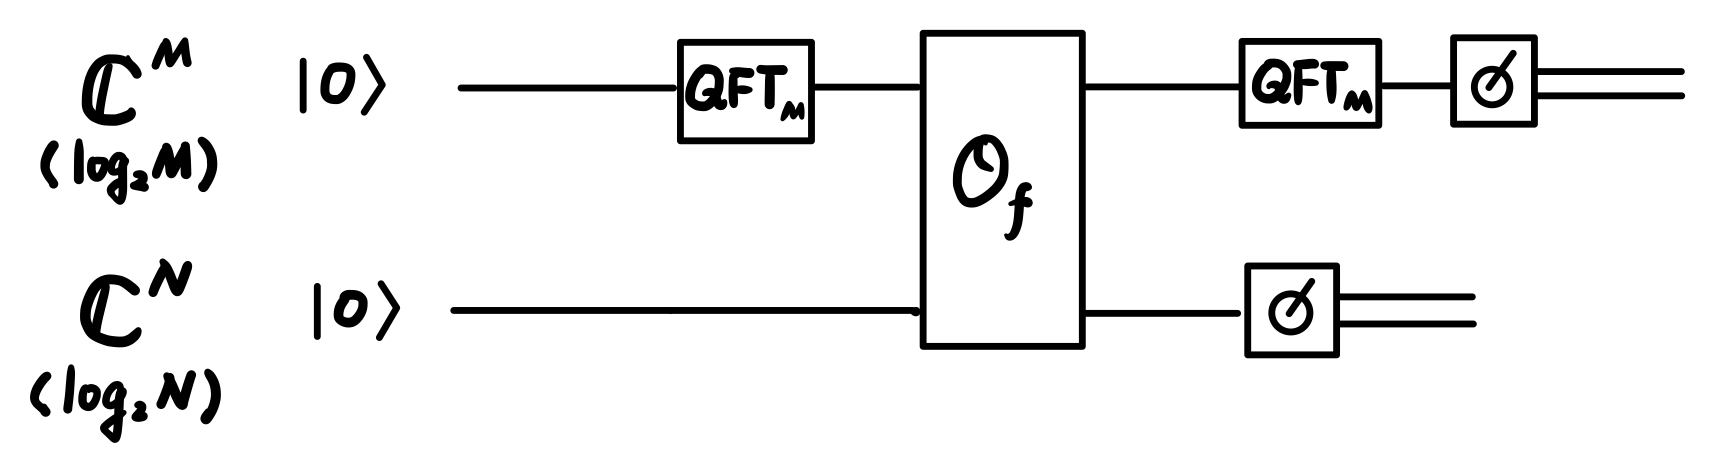
\includegraphics[scale = 0.2]{8/qft.png}
\end{center}
where we have:
\begin{align*}
    f: \{0, 1, 2, \dots, M-1\} &\to \{0, 1, \dots, N-1\} \\
    x &\mapsto a^x \bmod N
\end{align*}
We take $M > N^2$ and assume $M = \lambda r$ for some $\lambda \in \Z^+$. \\
After we measure the second qubit and obtain some $f(k)$ for $k \in \{0, 1, \dots, r - 1\}$, the first qubit collapes to:
$$\frac{1}{\sqrt{\lambda}} \Sum{l = 0}{\lambda - 1} \ket{k + l r}$$
where $l \in \{0, 1, \dots, \lambda - 1\}$. \\
After applying $\QFT$ on the first qubit, measurement on the first qubit, gives $n\lambda$ where $n$ is chosen u.a.r from $\{0, 1, \dots, r - 1\}$. \\
We extract $r$ by the following:
\begin{quote}
    1. Divide $n\lambda$ by $M$ to get $f := \frac{n}{r}$. \\
    2. Express $f$ in its simplest terms and read off the denominator, call $r'$. \\
    3. Verify if $a^{r'} \equiv 1 \bmod N$, if yes give $r'$, if not give ``fail''.
\end{quote}
There are two cases, if $n$ is co-prime to $r$, then $r' = r$, which occurs with probability $\ge \gamma$; if $n$ is not co-prime to $r$, $r$ is a multiple of $r'$. Then doing $\order{\frac{1}{\gamma}}$ repeats of the algorithm ensures with almost certainty that we land in the first case and obtain $r$. \\
The complexity of each repeat is $\order{\log^3 N}$ and $\frac{1}{\gamma} \sim \log(\log N)$. \\
The QFT circuit is implemented in the following way:
\begin{center}
    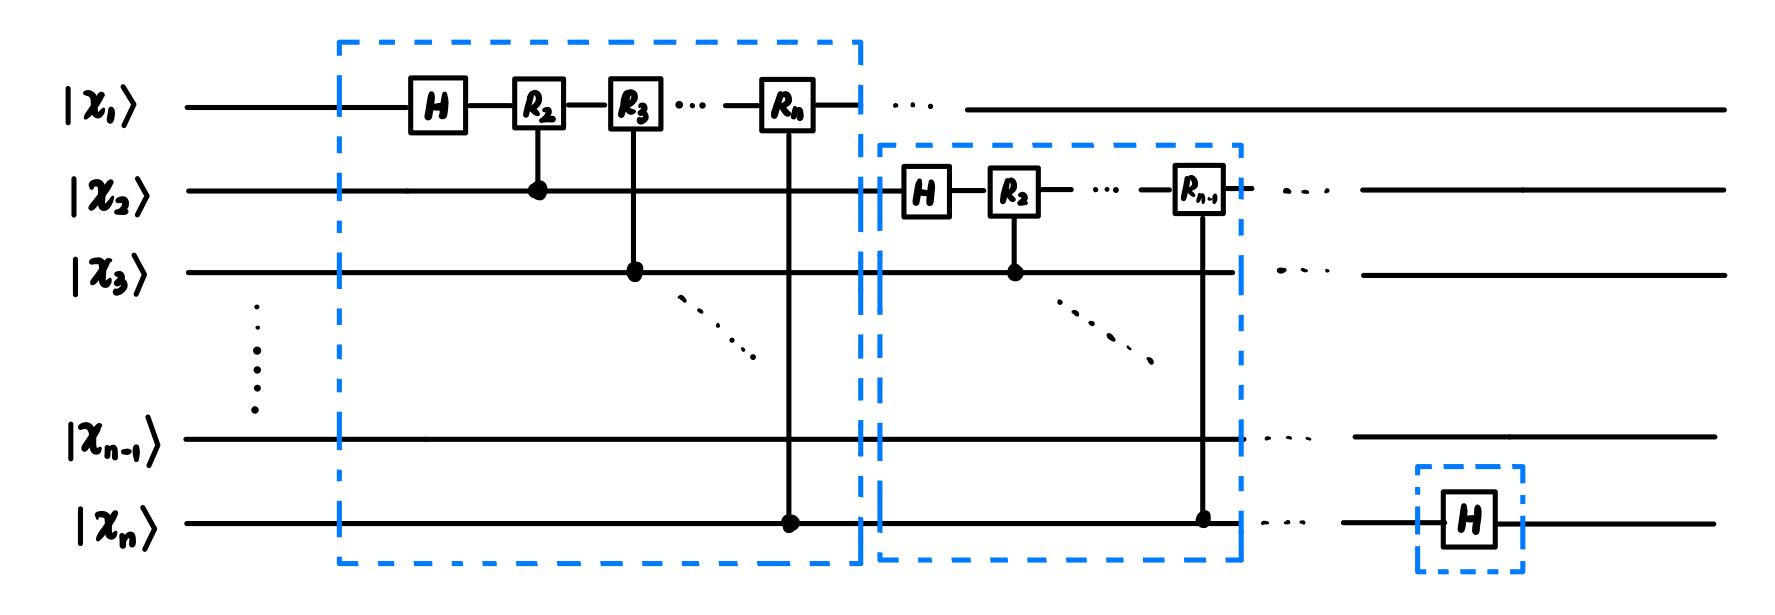
\includegraphics[scale = 0.2]{8/qft_circuit.png}
\end{center}
where
$$R_k = \begin{pmatrix}
    1 & 0 \\
    0 & e^{\imag \frac{2\pi}{2^k}}
\end{pmatrix}$$
This circuit is realized using $\order{n^2} \sim \order{\log^2 N}$ quantum gates.

\newpage
\section{Grover's Algorithm}
Grover's algorithm can be used to speed up the SAT problem. \\
Let
$$f: \binset^n \to \binset$$
we restrict it to
$$\begin{cases}
    f(\mathbf{x}) = 0 & \forall \mathbf{x} \in \binset^n \\
    f(\mathbf{x}) = 0 & \exists! \mathbf{x}^* \in \binset^n, f(\mathbf{x}^*) = 1
\end{cases}$$
The quantum circuit for Grover's algorithm is the following:
\begin{center}
    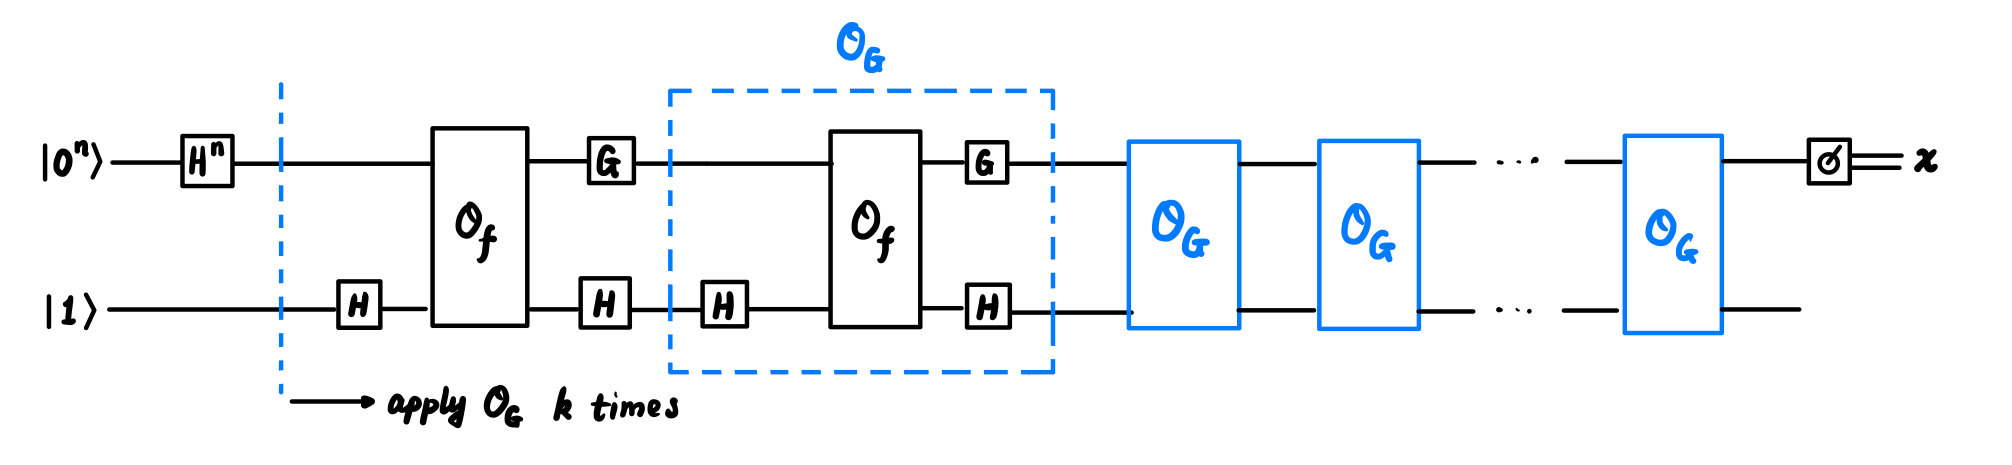
\includegraphics[scale = 0.2]{9/grover.png}
\end{center}
Recall the quantum phase oracle for $f$ is
$$\opuni_f = HO_fH: \ket{\mathbf{x}} \ket{b} \mapsto (-1)^{b \cdot f(\mathbf{x})} \ket{\mathbf{x}}\ket{b}$$
We define $V_f$ where (take $b = 1$ for $\opuni_f$)
$$V_f: \ket{\mathbf{x}} \mapsto (-1)^{f(\mathbf{x})}\ket{\mathbf{x}}$$
and define:
$$\ketpsi = \frac{1}{\sqrt{2^n}}\Sumi{\mathbf{x}}\ket{\mathbf{x}}$$
$$G := \id - 2\op{\psi}$$
The state before measurment in this setup is essentially
$$(GV_f)^kH^n\ket{0^n}$$
In the first case, this becomes $(-1)^k \ketpsi$. \\
In the second case, $\ketpsi$ can be written as:
$$\ketpsi = \sqrt{\frac{N - 1}{N}} \ket{\psi_0} + \sqrt{\frac{1}{N}} \ket{\psi_1} = \cos \theta \ket{\psi_0} + \sin \theta \ket{\psi_1}$$
where $N = 2^n$, and
$$\ket{\psi_{0}} = \frac{1}{\sqrt{N -1}} \Sumi{\mathbf{x} \ne \mathbf{x}^*} \ket{\mathbf{x}}$$
$$\ket{\psi_1} = \ket{\mathbf{x}^*}$$
We can calculate $-GV_f$ with respect to $\ket{\psi_0}$ and $\ket{\psi_1}$ to be:
$$\begin{pmatrix}
    \cos 2\theta & -\sin 2\theta \\
    \sin 2\theta & \cos 2\theta
\end{pmatrix}$$
which is rotating $2 \theta$ counterclockwise. \\
In the second case, $\ketpsi$ starts with a $\theta$ between it and the $\ket{\psi_0}$ axis, and after applying $-GV_f$ $k$ times, we want it to be close to $\ket{\psi_1}$. This means:
$$(2k + 1)\theta = \frac{\pi}{2} \to k \approx \frac{\pi}{4}\sqrt{N}$$
(Soufflé problem: fixed point amplification)

\subsection{Limitations of Quantum Algorithm in Query Models}
We demonstrate that if a quantum computer can only query $f$, it must use $\Omega(\sqrt{2^n})$ queries to decide if $f$ maps $\mathbf{x}$ to $1$. \\
We consider a general model of any quantum algorithm:
\begin{center}
    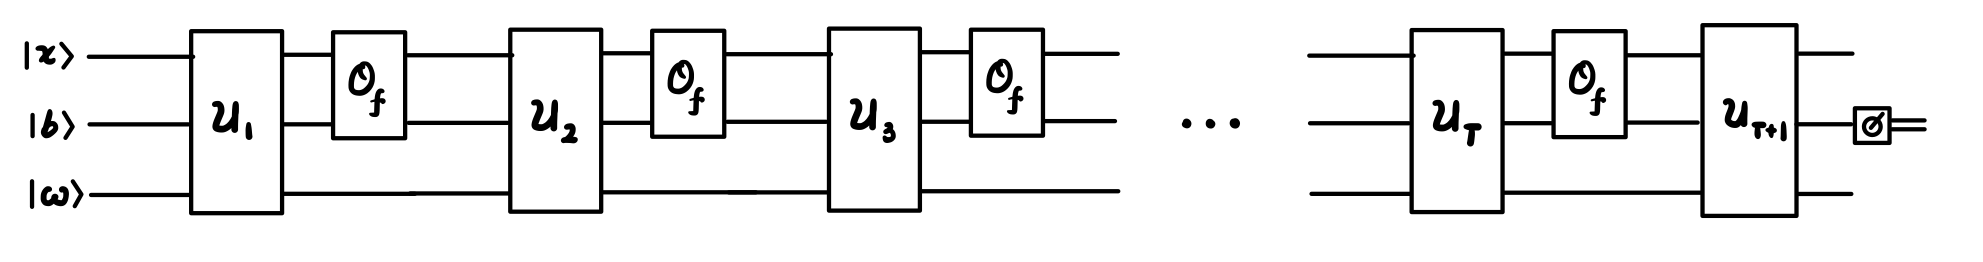
\includegraphics[scale = 0.2]{9/general_qc.png}
\end{center}
Here, $T$ represents the number of queries to $f$. \\
We consider the circuit for different choices of $f$, denote the circuit where $f$ maps everything to $0$ to be ``0'', $f$ maps $\mathbf{x}_i$ to $1$ and the rest to $0$ to be ``$\mathbf{x}_i$''. \\
The limitation is that if $T$ is small, the algorithm can ``look at'' at most $T^2$ values of $f(\mathbf{x})$, and if $T^2 < N$, there will exist $\mathbf{x}^* \ne \mathbf{x}_i$ such that the output of circuit ``0'' is indistinguishable from ``$\mathbf{x}^*$''.
\begin{center}
    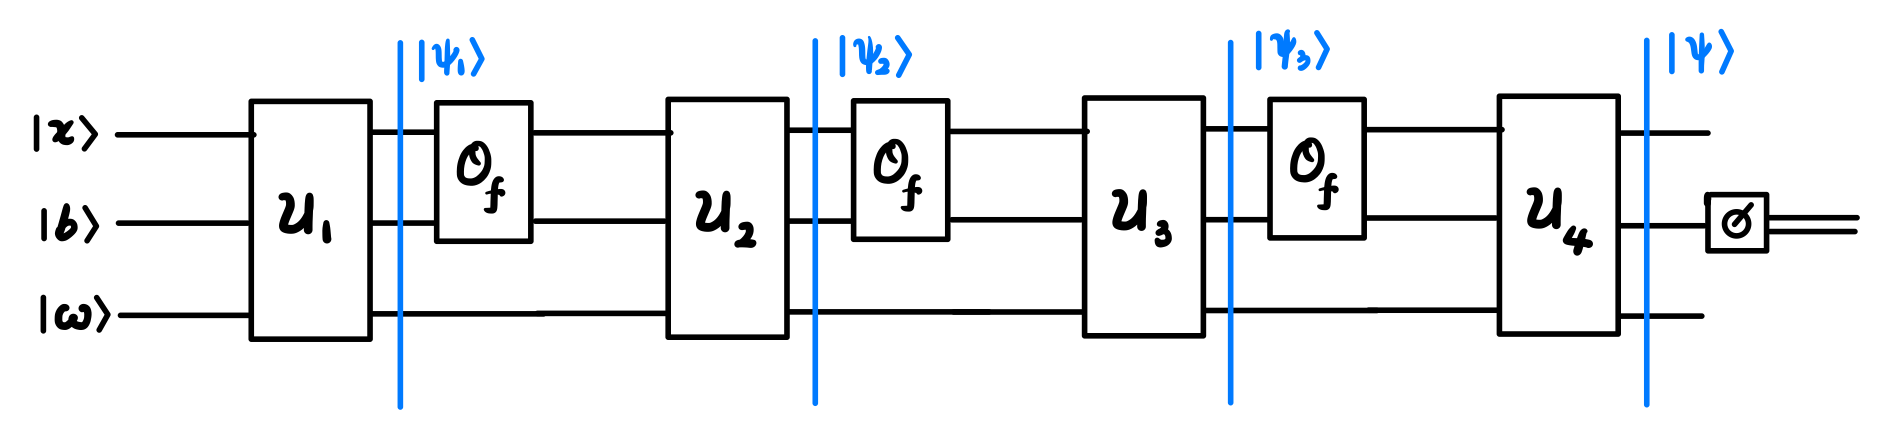
\includegraphics[scale = 0.2]{9/3-step.png}
\end{center}
Let $t \in \{1, \dots, T\}$ and $\ket{\psi_t}$ be the state for $t$th query, we write:
$$\ket{\psi_t} = \Sumi{\mathbf{x}, b, \omega} \alpha_{\mathbf{x}, b, \omega}^t \ket{\mathbf{x}, b, \omega}$$
where $t$ is just a \textbf{superscript}. \\
Let
$$Q_\mathbf{x}^t = \Sumi{b, \omega} \abs{\alpha_{\mathbf{x}, b, \omega}^t}^2$$
$$Q_\mathbf{x} = \Sum{t = 1}{T} Q_\mathbf{x}^t$$
Then, by expanding the terms:
$$\Sumi{\mathbf{x}}Q_\mathbf{x} = T$$
there must exist $x^*$ such that $Q_{\mathbf{x}^*} \le \frac{T}{N}$. This means, if $T < \sqrt{N}$, the quantum circuit cannot distinguish circuit ``0'' from circuit ``$\mathbf{x}^*$''. \\
We show this by considering a function, $g: \binset^n \to \binset$ such that $g(\mathbf{x}^*) = 1$ and $g(\mathbf{x}) = 0$ for $\mathbf{x} \ne \mathbf{x}^*$.
\begin{theorem}
    Let $\ket{\gamma}$ be the state of circuit ``$\mathbf{x}$'' just before measurement, Then
    $$\norm{\ketpsi - \ket{\gamma}} \le 2 \Sum{t = 1}{T} \sqrt{Q_{\mathbf{x}^*}^t}$$
\end{theorem}
The idea behind this is that we first replace the last $f$ from circuit ``0'' with $g$ and bound the difference. Then replace the last two $f$ from circuit ``0'' with $g$ and bound the difference. Eventually, we replace all $f$ with $g$ and bound the difference.
\begin{theorem}
    At time step $t$, we replace the last $T - t + 1$ $f$ with $g$, and we can show that at each replacement, the difference between states just before measurement is bound by $4Q_{\vecx}^t$
\end{theorem}
Then:
\begin{align*}
    \norm{\ketpsi - \ket{\gamma}} &\le 2 \Sum{t = 1}{T} \sqrt{Q_\vecx^t} \\
    &= 2 \Sum{t = 1}{T} 1 \cdot \sqrt{Q_\vecx^t} \\
    &\le 2 \sqrt{T} \sqrt{\Sum{t = 1}{T} Q_\vecx^t} \\
    &= \frac{2T}{\sqrt{N}}
\end{align*}
which is small unless $T \ge \Omega(\sqrt{N})$.

\newpage
\section{Quantum Error Detection and Correction - 量子错误探测与改正}
\subsection{Classical Error Correction}
The fundamental idea of error detection and correction is to \impt{add redundancy to data to project against errors}. \\
The simplest classical code is ``repetition code'', where we code $0$ as $000$ and $1$ as $111$. We can detect and correct any single bit flip. The rate of this method is $\frac{1}{3}$. \\
Another classical method is the Hamming code, where we code $4$ bits into $7$ bits, with the rate of $\frac{4}{7}$. This is achieved by
$$p_1 = d_1 \oplus d_2 \oplus d_3$$
for one of the error detection code. \\

\subsection{Quantum Error Detection and Correction}
A na\"ive generalization of the repetition code does not work in quantum, the operation:
$$\ketpsi \mapsto \ketpsi\ketpsi\ketpsi$$
is not possible to due \impt{no-cloning principle}.
\begin{definition}
    A $d$-dimensional \uimpt{observable} $\mathcal{O}$ is a $d \times d$ \impt{Hermitian} matrix where $\conjt{\mathcal{O}} = \mathcal{O}$.
\end{definition}
An $n$-qubit observable is a $2^n$-dimensional observable.
\begin{definition}
    Let $\mathcal{O}$ be an $n$-qubit observable, $\ketpsi$ is an $n$-qubit state, suppose $\mathcal{O}\ketpsi = \lambda\ketpsi$ for some $\lambda \in \R$, then \uimpt{measuring} $\mathcal{O}$ on $\ketpsi$ refers to a process that returns $\lambda$ and the state remains $\ketpsi$.
\end{definition}
\begin{definition}
    An $n$-qubit \uimpt{stabilizer} (Pauli operators) is a $2^n \times 2^n$ matrix of form $P_1 \otimes P_2 \otimes \cdots \otimes P_n$, where $P_i \in \{\id, X, Y, Z\}$
\end{definition}
When we measure a stabilizer on an eigenstate, we will obtain outcomes in $\{+1, -1\}$.
\begin{definition}
    If $A, B$ are complex matrices of same dimensions, we say $A, B$ \uimpt{commute} if $AB = BA$ and \uimpt{anti-commute} if $AB = -BA$.
\end{definition}
This gives that any two stabilizers commute or anti-commute. \\
A set of $k$ stabilizers can be \impt{simultaneously} measured if $\mathcal{S}_i$ commutes with $\mathcal{S}_j$. This is a ``physical interpretation'' of the mathematical fact that a set of commuting diagonalizable matrices can be simultaneously diagonalized.
\begin{lemma}
    Let $\ketpsi$ be an $n$-qubit state and $P$ an $n$-qubit stabilizer, and $\opuni$ an $n$-qubit unitary, if $P\ketpsi = \ketpsi$ ($P$ stabilizes $\ketpsi$), and $P\opuni = \alpha \opuni P$, for $\alpha \in \{+1, -1\}$, then measuring $P$ on $\opuni\ketpsi$ gives outcome $\alpha$.
\end{lemma}

\subsubsection{Bit-flip Error}
Analogous to the repetition code, we encode a state $\ketpsi = \alpha \ket{0} + \beta \ket{1}$ to be $\ket{\psi'} = \alpha\ket{000} + \beta\ket{111}$, where $\ket{000} := \ket{0_L}$ and $\ket{111} = \ket{1_L}$ (``L'': logical encoding). \\
This is achieved through the circuit:
\begin{center}
    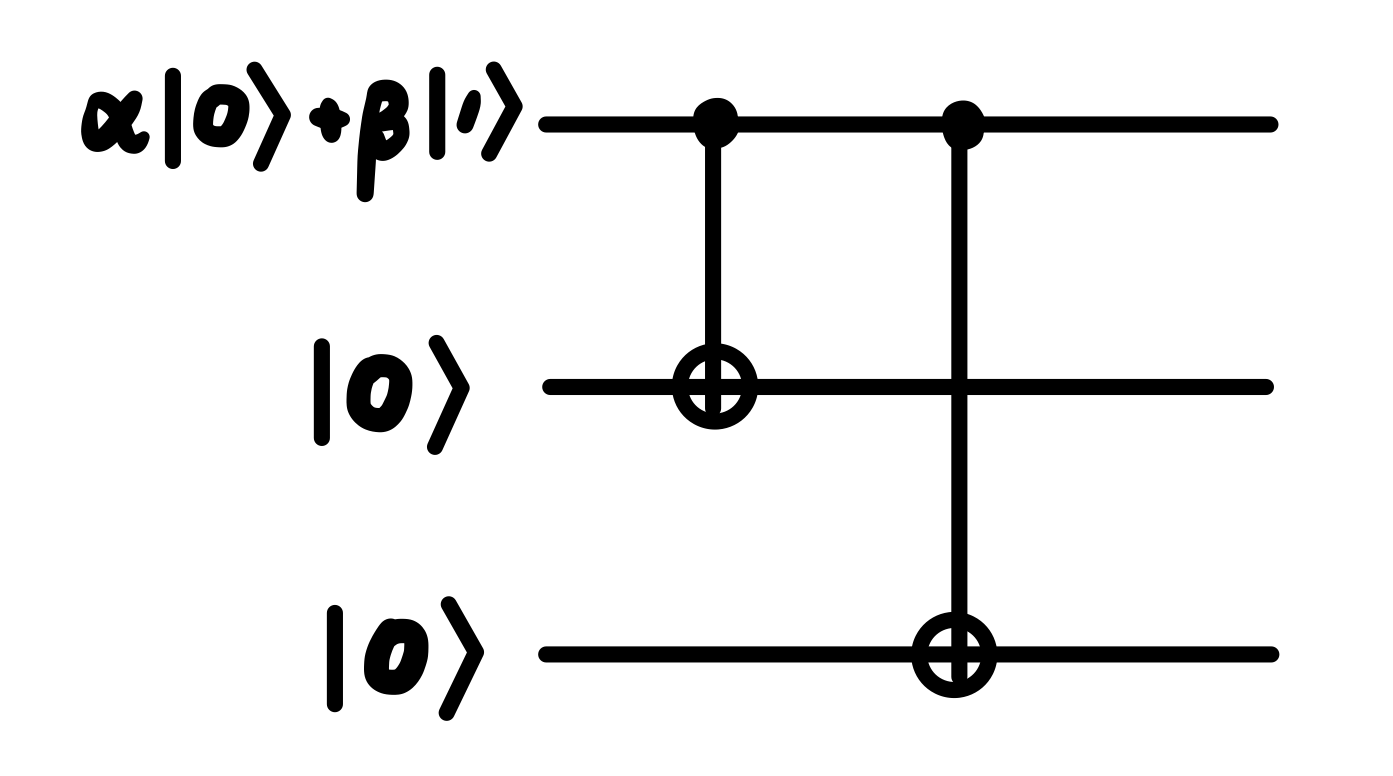
\includegraphics[scale = 0.2]{10/bitflip.png}
\end{center}
This protects against any single-qubit flip. We can detect and correct the errors by measuring:
\begin{align*}
    Z_1Z_2 &= Z \otimes Z \otimes \id \\
    Z_2Z_3 &= \id \otimes Z \otimes Z
\end{align*}
If we measure to $(+, +)$, there is no error. If we measure to $(-, +)$, the first qubit is flipped. If we measure to $(-, -)$, the second qubit is flipped. If we measure to $(+, -)$, the third qubit is flipped. We call this the ``error syndrome table''. \\
However, this cannot detect phase flips.

\subsubsection{Phase-flip Error}
We encode a state $\ketpsi = \alpha \ket{0} + \beta \ket{1}$ to be $\ket{\psi'} = \alpha\ket{+++} + \beta\ket{---}$, where $\ket{+++} := \ket{0_L}$ and $\ket{---} = \ket{1_L}$ through the circuit:
\begin{center}
    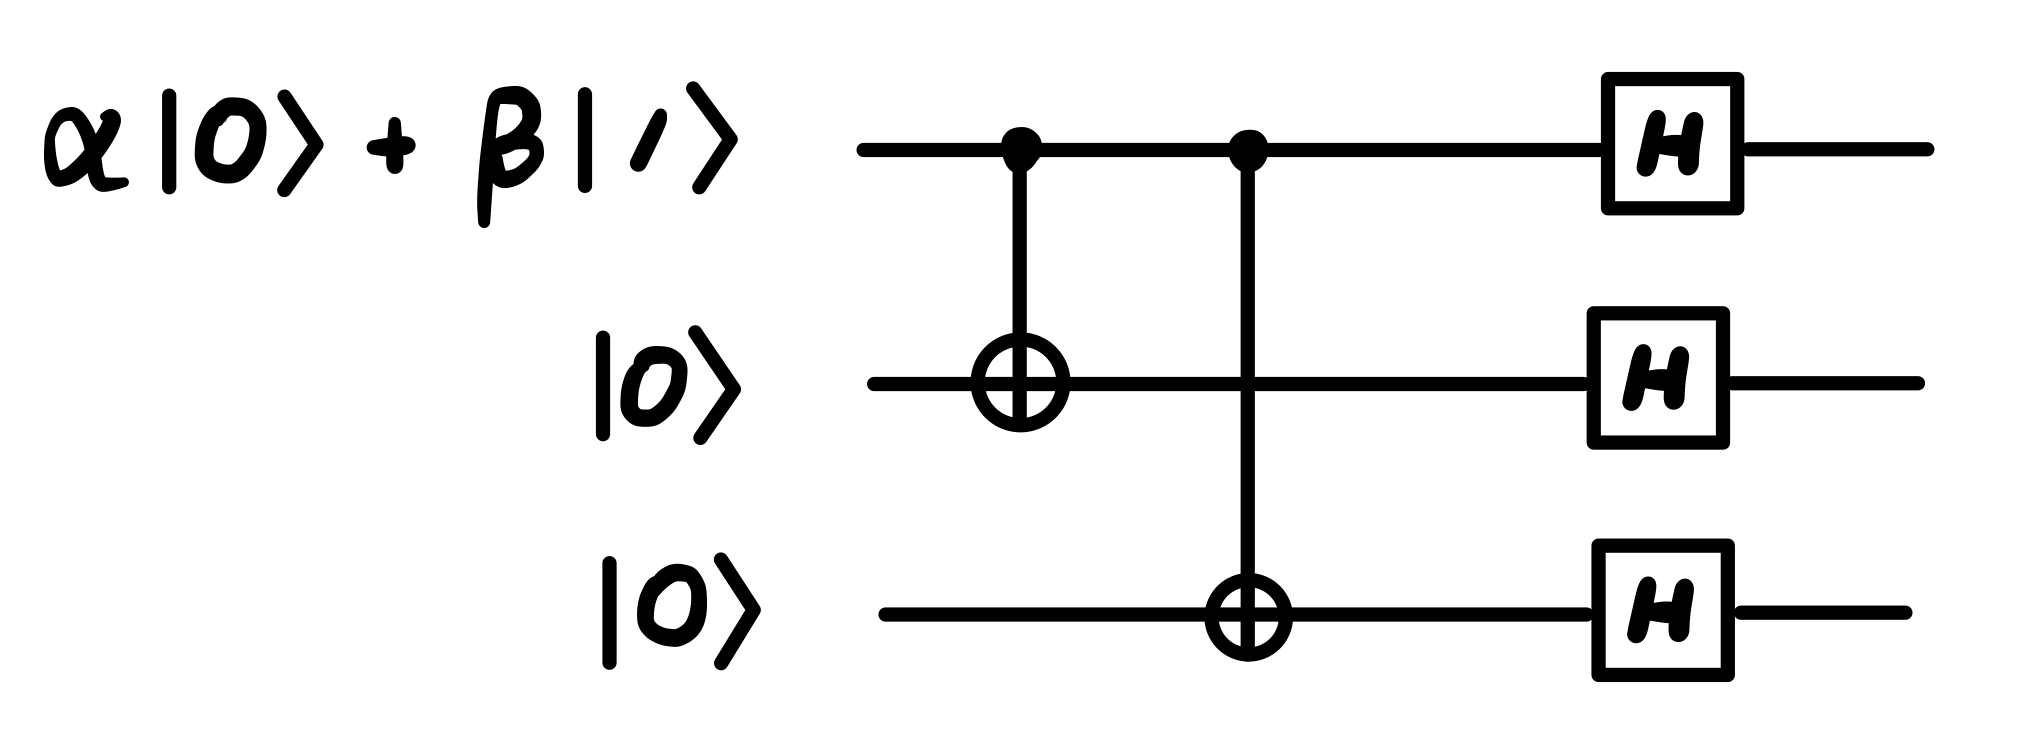
\includegraphics[scale = 0.2]{10/phaseflip.png}
\end{center}
We then measure $(X_1X_2, X_2X_3)$. Analogous to previous section, this can detect any single-qubit phase flip, not any single-qubit bit flip.

\subsubsection{Shor's Code}
One way to detect both bit flips and phase flips on a single-qubit is to use $9$-qubit Shor's code, where it is achieved by the circuit:
\begin{center}
    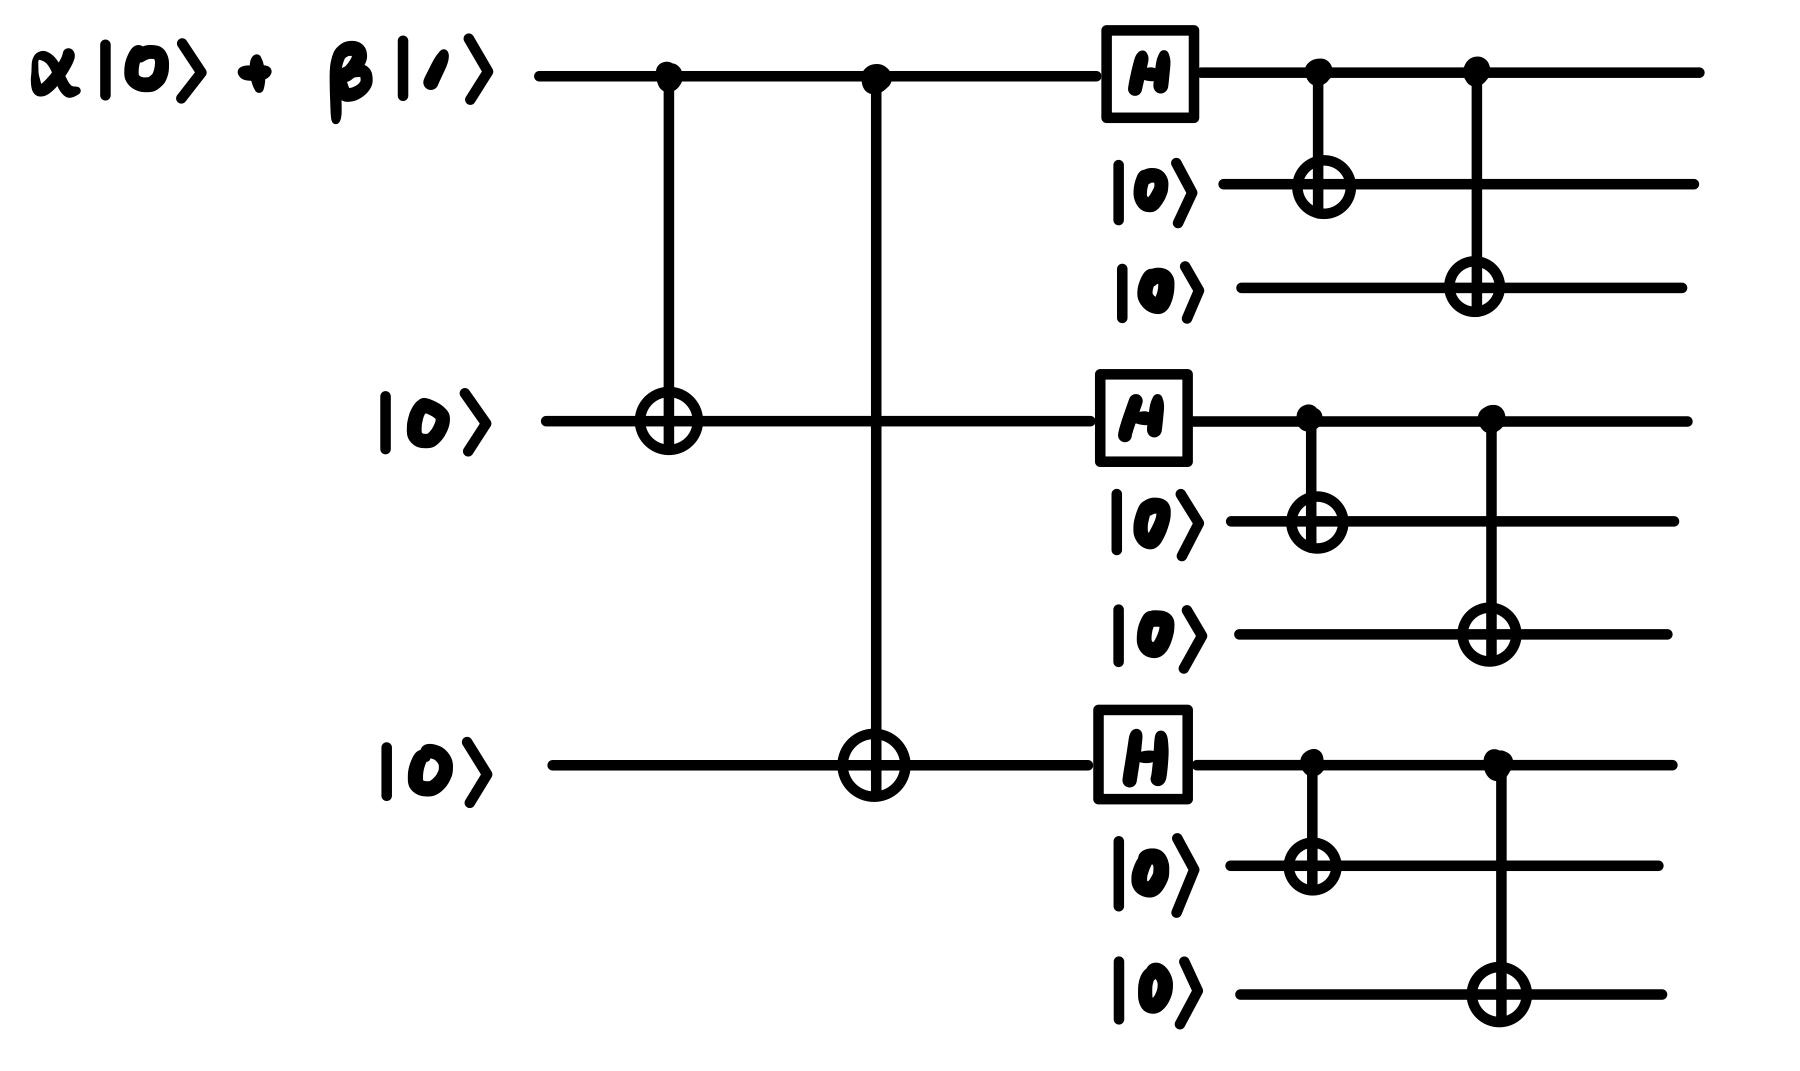
\includegraphics[scale = 0.2]{10/bothflip.png}
\end{center}
And the logical encoding is that
\begin{align*}
    \ket{0_L} &:= \frac{1}{2\sqrt{2}}(\ket{000} + \ket{111})(\ket{000} + \ket{111})(\ket{000} + \ket{111}) \\
    \ket{1_L} &:= \frac{1}{2\sqrt{2}}(\ket{000} - \ket{111})(\ket{000} - \ket{111})(\ket{000} - \ket{111})
\end{align*}
The corresponding stabilizers are:
$$(Z_1Z_2, Z_2Z_3),(Z_4Z_5, Z_5Z_6)(Z_7Z_8, Z_8Z_9)$$
and
$$(X_1X_2X_3X_4X_5X_6, X_4X_5X_6X_7X_8X_9)$$
Even though Shor's code's error syndrome table has non-distinct columns, we can still correct any single qubit error. \\
For example, the columns $Z_1, Z_2, Z_3$ (error gates) will be the same, if we observe the common syndrome of $Z_1, Z_2, Z_3$, we can still correct by multiplying the state by $Z_1$.
\begin{quote}
    1. Error was $Z_1$: $Z_1(Z_1\ketpsi) = \ketpsi$. \\
    2. Error was $Z_2$: $Z_1(Z_2\ketpsi) = (Z_1Z_2)\ketpsi = \ketpsi$ as $Z_1Z_2$ is a stabilizer. \\
    3. Error was $Z_3$: $Z_1(Z_3\ketpsi) = (Z_1Z_2)(Z_2Z_3)\ketpsi = \ketpsi$
\end{quote}
We can identify the block on which the error occurred:
\begin{quote}
    1. if the $Z$ rows have $-$ signs, $1-3$ are the first block, $4-6$ are the second block, and $7-9$ are the third block, with $X, Y$ errors. \\
    2. if the $X$ rows take value $(-, +)$, it's first block; if $(-, -)$, it's second block; if $(+, -)$, it's third block.
\end{quote}
If a QEC can correct any single-qubit $X,Y,Z$ errors, then it can correct ``arbitrary'' single-qubit errors.

\subsection{How to Measure Stabilizers}
We can measure say $\id \otimes X \otimes Y \otimes Z$ on a $4$-qubit state $\ketpsi$ in the following way:
\begin{center}
    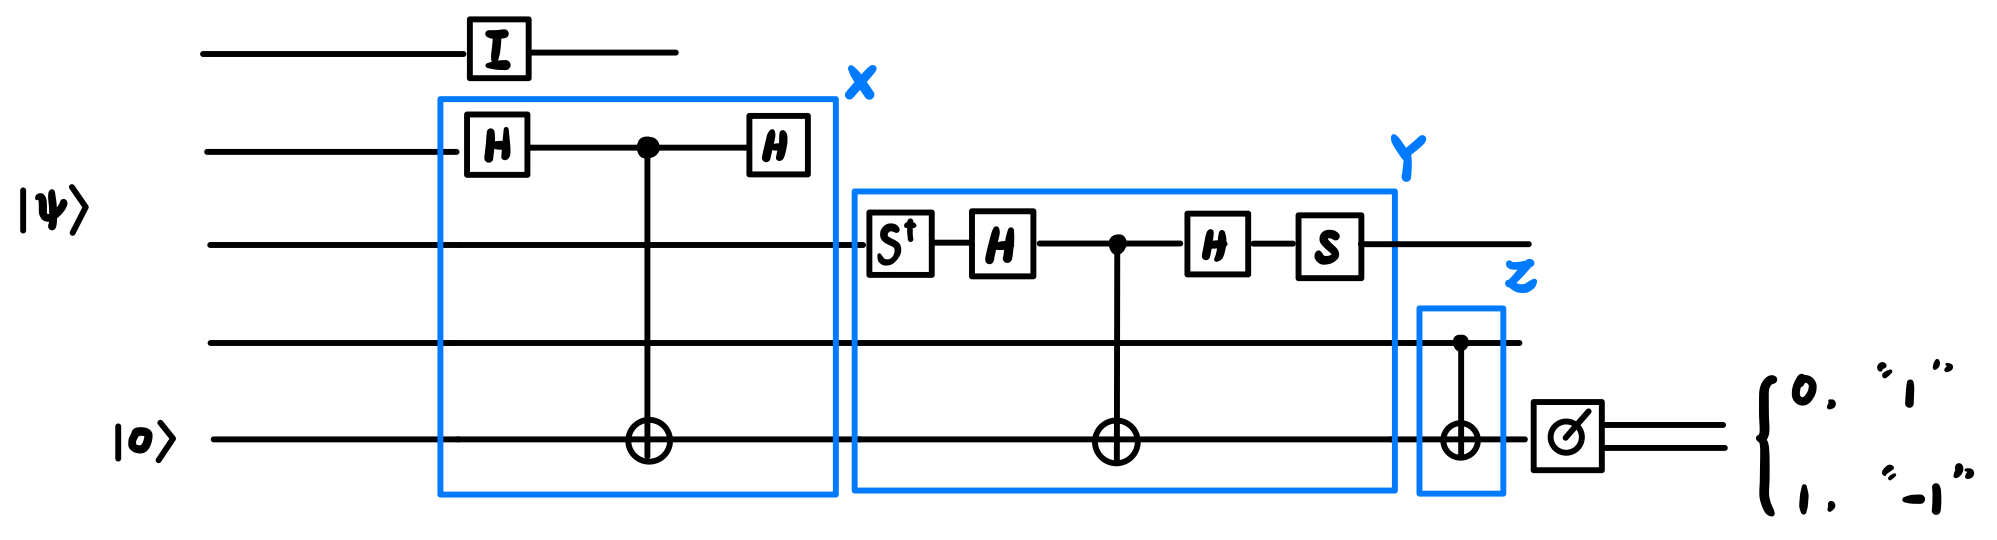
\includegraphics[scale = 0.2]{10/stabilizer.png}
\end{center}

\end{document}